\documentclass[11pt]{article}
\usepackage{graphicx}
\usepackage{epic}
%%% displayed synchronous programs
\makeatletter
\def\BEP{\begin{trivlist}\item[]
  \if@minipage\else\vskip\parskip\fi
  \leftskip\@totalleftmargin \advance\leftskip by 1\parindent
  \rightskip\z@ \parindent\z@ \parfillskip\@flushglue \parskip\z@
  \@tempswafalse \def\par{\if@tempswa\hbox{}\fi\@tempswatrue\@@par}
  \obeylines \tt \small \catcode``=13 \@noligs\frenchspacing\@vobeyspaces}
\def\EEP{\end{trivlist}}
\makeatother

\def\pp#1{\texttt{\small{#1}}}
\newcommand{\PP}[1]{\noindent{\textit{\textbf{#1}}}}

\def\X#1{$x_{#1}$}
\def\B#1{\texttt{#1}}

\def\se{\textit{syn{\small ERJY}}}
\def\sec{\textit{syn{\small ERJYcharts}}}
\def\sef{\textit{syn{\scriptsize ERJY}}}
\def\argos{\textsc{Argos}}
\def\lustre{\textsc{Lustre}}
\def\signal{\textsc{Signal}}
\def\esterel{\textsc{Esterel}}
\def\statecharts{\textsc{Statecharts}}
\def\synccharts{\textsc{SyncCharts}}
\def\java{\textsc{Java}$^{\mbox{\tiny TM}}$}
\def\matlab{\textsc{MATLAB}$^{\mbox{\tiny TM}}$}

\newcommand{\GO}[0]{{\small GO}}
\newcommand{\GOs}[0]{{\small GO}s}
\newcommand{\spc}[0]{\vspace{0.2cm}}

\newcommand{\vs}[0]{\vspace{1pt}}
\newcommand{\NTI}[1]{\textit{#1}}
\newcommand{\NTD}[1]{{\em #1}\label{#1}}
\newcommand{\NT}[1]{\index{#1@{\em #1}}\hyperref{#1}{#1}{}{#1}}
\newcommand{\NTZ}[2]{\index{#1@{\em #1}}\hyperref{#1}{#1#2}{}{#1}}
\newcommand{\KWI}[1]{{\index{#1@{\tt #1}}\tt #1}}
\newcommand{\T}[1]{{\tt #1}}
\newcommand{\is}[0]{$\Rightarrow$\vs}
\newcommand{\mto}[0]{$\mapsto$}
\newcommand{\Bopt}[0]{{\bf (}}
\newcommand{\optE}[0]{{\bf )\opt}}
\newcommand{\opt}[0]{$_{\textit{\scriptsize opt~}}$}
\newcommand{\Balt}[0]{{\bf (}}
\newcommand{\alt}[0]{\,$|$}
\newcommand{\altE}[0]{{\bf )$_\mbox{\em alt~}$}}
\renewcommand{\altE}[0]{{\bf )~}}
\newcommand{\lst}[0]{{...~~}}
\newcommand{\lsep}[1]{...\fbox{\scriptsize #1}...~~}
\newcommand{\rr}[0]{\vs\makebox[7mm]{}}

\newtheorem{example}{\bf Example}[section]
\newenvironment{BNF}{}{}

\def\codeinput#1{\IfFileExists{../tex_input/se.#1}{\input ../tex_input/se.#1}{\begin{center}chpt\_\thechapter\_#1.se\end{center}} {\footnotesize(cf. \texttt{chpt\_\thechapter\_#1.se})}}

\def\codefragment#1{\IfFileExists{../tex_input/se.#1}{\input ../tex_input/se.#1}{\begin{center}chpt\_\thechapter\_#1.se\end{center}}}

\def\codeinputref#1{\IfFileExists{../tex_input/se.#1}{\input ../tex_input/se.#1}{\begin{center}ref\_#1.se\end{center}} {\footnotesize(cf. \texttt{ref\_#1.se})}}

\def\codeinputuser#1{\IfFileExists{../tex_input/se.#1}{\input ../tex_input/se.#1}{\begin{center}user\_#1.se\end{center}} {\footnotesize(cf. \texttt{user\_#1.se})}}

\def\A{\mbox{${\cal A}$}}
\def\C{\mbox{${\cal C}$}}
\def\D{\mbox{${\cal D}$}}
\def\E{\mbox{${\cal E}$}}
\def\F{\mbox{${\cal F}$}}
\def\H{\mbox{${\cal H}$}}
\def\I{\mbox{${\cal I}$}}
\def\L{\mbox{${\cal L}$}}
\def\M{\mbox{${\cal M}$}}
\def\P{\mbox{${\cal P}$}}
\def\Q{\mbox{${\cal Q}$}}
\def\R{\mbox{${\cal R}$}}
\def\S{\mbox{${\cal S}$}}
\def\V{\mbox{${\cal V}$}}

\def\ARROW#1#2{\mbox{\def\arraystretch{0.1}\begin{tabular}{c}
$\ \scriptstyle #1\ $\\
\rightarrowfill\\
$\ \scriptstyle #2\ $\end{tabular}}}

\def\mkTitle#1{
\title{
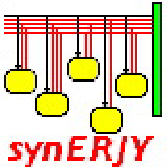
\includegraphics[height=50pt]{../pdf/se-logo}\hspace{0.5cm}
{\Huge \textit{\textbf{synERJY} 5.3}} \\ \vspace{1cm}\
       \textbf{#1}}

\author{\textit{Reinhard Budde}\\
\textit{Axel Poign\'e}\\
\textit{Karl-Heinz Sylla}\\
\ \\
\textbf{Fraunhofer Institut}\\\ \\ 
\textbf{Autonome intelligente Systeme}\\\ \\
\textbf{Fraunhofer AiS}\\\ \\\ \\
\\\ \\\ 
\\\  \\\ \\\ \\\ \\\ \\\textbf{\Large }
}

\date{\today}
}

\makeindex

\mkTitle{Using the Programming Environment}

\begin{document}

\maketitle


\section*{Preface}

\se\footnote{\sef\ may be read as \textbf{syn}chronous
\textbf{e}mbedded \textbf{r}eactive \textbf{J}ava with a \textbf{y}
for the sound.} is a programming language and a design environment for
embedded reactive systems that combines two paradigms:
\begin{itemize}
    \item \emph{Object-oriented modelling} for a robust and flexible
    design.
      
    \item \emph{Synchronous execution} for precise modelling of
    reactive behaviour.
\end{itemize}
Highlights are that
\begin{itemize}
\item \se\ provides a deep embedding of the reactive behaviour into
      the object-oriented data model.
\item \se\ offers fine-grained integration of synchronous formalisms
      such as \esterel~\cite{esterel}, \lustre~\cite{lustre}, and
      \statecharts~\cite{statecharts}.\footnote{We recommend Halbwachs' book
      \emph{Synchronous Programming of Reactive Systems}~\cite{halbwachs} as 	an excellent introduction.}
\end{itemize}

The programming environment supports compilation, configuration,
simulation, and testing, as well as verification by model checking. 
Behavioural descriptions may be edited in graphical or in textual
form.  Code generators for efficient and compact code in C and several
hardware formats are available.

The \se\ language and its programming environment are developed
at the Fraunhofer Institut Autonome Intelligente Systeme.\footnote{The
development of \sef\ has been partially supported by the ESPRIT LTR
SYRF, ``Synchronous formalisms'', and the ESPRIT IIM Project CRISYS,
``Critical Systems and Instrumentation''.}  The programming
environment is freely available with a public domain license.
\newline

\noindent Contact:  
{\tt\small \{reinhard.budde,poigne,sylla\}@ais.fraunhofer.de}.



\newpage
\tableofcontents

\newpage

\section{Overview}\label{PE}

The \se\ programming environment consists of three components. 

\begin{itemize}
    \item \textbf{\se\ Console}: the compiler bundled with a general
    control panel for the \se\ programming environment. 

    \item \textbf{\se\ Simulator}: the step through simulation tool.

    \item \textbf{\se\ Graphic Editor}: the visual editor for
    hierarchical automata.
\end{itemize}

\se\ is a public domain software available at
\begin{center}
\pp{www.ais.fraunhofer.de/\~{}ap/synERJY}
\end{center}
for Linux, Windows XP, and MacOS X. Target system generation depends on the availability of cross compilers. The present distribution supports system generation from Linux to the Hitachi Hi8 processor (used in the LEGO Mindstorms controller RCX) and some Atmel AVR micro controllers, MPC555, and some Texas Instrument DSPs. Example programs are included in the distribution.

\section{Installation}

\begin{description}
\item[\textbf{Windows XP}]\ \\
 \texttt{synERJY.exe} installs the basic \se\ environment. Just run the executable and tick boxes as appropriate. Other set-up executables are provided for specific target architectures.

\item[\textbf{Linux}]\ \\
Untar the distribution, and move the {\tt synERJYlinux} distribution wherever
appropriate. Then set the environment variable {\tt SE\_HOME} to {\ .../synERJY}.

\item[\textbf{Mac OSX}]\ \\
Untar the distribution, and move the {\tt synERJYdarwin} distribution wherever
appropriate. Then set the environment variable {\tt SE\_HOME} to {\ .../synERJY}.

\end{description}


\section{Getting Started}\label{GetStarted}

\paragraph{Running the environment.} Copy an example program, e.g.
\pp{basic1.se} from the \pp{target/host/examples}
(resp. \pp{target$\backslash$host$\backslash$examples}) directory of the \se\
distribution to some working directory. Preview the example file using your favourite editor\footnote{A syntax definition file for \se\ is provided for vim :-)}. Start the \se\ console 
\begin{description}
\item[\textbf{Windows XP}]\ \\
 by double-clicking on the file \pp{basic1.se} in the directory\\
  \pp{$\ldots\backslash$examples$\backslash$Basic1}. 
\item[\textbf{Linux}]\ \\
  by calling the command \pp{synERJY} in a shell, and then loading the
   project \pp{\ldots/Basic1}.
\item[\textbf{Mac OSX X11 version}]\ \\
  as for Linux.
\end{description}

\paragraph{Loading a project.} Use the \textsf{File}$\mapsto$\textsf{Load project} menu entry\footnote{Shortcuts are indicated in the menus by
letters. We use \pp{Ctrl-<Key>} for invocation.} to start the
load-project-dialog. Select the project \pp{Basic1}. The project is loaded and
the configuration class defined in the file \pp{basic1.se} is compiled
and added to the database of the compiler.
Change the source file using your favourite editor. Now you may
re-compile the project by using the \textsf{File}$\mapsto$\textsf{Reload} menu
entry. Even easier is to click the \textsf{reload}-button on the left hand side
of the console window. Note, that the name \pp{Rc} of the configuration class
contained in the file \pp{basic1.se} becomes the name of the configuration
class in the console window. As you may guess, this class has a static method
\pp{main} to start the application.
 

\paragraph{Code generation for Simulation.} Now you may want to generate code for
simulation. \se\ can generate code to be used with the simulator only, if
a C compiler for the operating hosting the \se\ environment is available. All
different flavours of UNIX have \pp{gcc}, some UNIXes have other C-compiler,
too. For win32 systems either a licence for VisualStudio must be
available, or public domain software must be installed which features a
C-compiler, for instance \pp{Cygwin} or \pp{Mingw32/MSys}. The operating system
MacOS X used for the Apple Macintosh has a \pp{gcc} compiler. By either selecting
the \textsf{Make}$\mapsto$\textsf{Build} menu entry or by
clicking the \textsf{Build} button the compiler generates C code and
then calls the C compiler to compile and link the object file against a small
runtime library which is part of the \se\ distribution. If only C code is to be
generated, use \textsf{Make}$\mapsto$\textsf{Compile}. Then the \textsf{Build} button 
will be renamed to \textsf{Compile} with according behaviour. Using  
\textsf{Make}$\mapsto$\textsf{Build} toggles again.

The C-code generated by the \se\ compiler is stored in the temporary files
\pp{se.sim.Rc.h} and \pp{se.sim.Rc.c}. Remember, that \pp{Rc} is the name of the
configuration class from the file \pp{basic1.se}. All temporary files are
prefixed with \pp{se.}. If you do not use filenames starting
with this prefix by yourself, it is safe to remove temporary files
by \pp{rm se.*}.

\paragraph{Simulation} By selecting either the
\textsf{Utils}$\mapsto$\textsf{Simulator} menu entry or by clicking the
\textsf{Simulator}-button the simulator is started. You may trigger an instant
by clicking the \textsf{React} button. By clicking an input signal it will be
present in the next reaction. Make input signals present, trigger an
instant, look at the source code and check whether that happened what you
expected :-). You may edit the source and look for effects. Now we have stepped
through one elementary debugging cycle. For generating code for a target
micro-controller see section~\ref{simTgt}.


\section{The synERJY Programming Environment}\label{se-console}

\subsection{The Console}
The \se\ \emph{console} controls the compilation of \se\ programs and allows to
call other components of the programming environment. The \se\ compiler
maintains a database in which all classes from all files which have been loaded
during the actual session are stored. \se\ programs can be composed from
different files, of course. But: as the database indicates, there is no means
for separately storing the compiler outcome of a single compilation (into a
\pp{.o} file e.g. Such a feature is usually called separate compilation). This
is intentionally: The \se\ compiler does a lot of global optimisations before
code is generated: for example, class hierarchy analysis to replace dynamic by
static binding of methods calls, if possible.  Thus a typical development cycle
is: load a project, generate code, simulate, edit a file to remove an error,
re-load that file only, generate code, simulate, and so on.

Fig.~\ref{console-screenshot} is a screen-shot of the console window after
loading a file and generating simulation code.

\begin{figure}[h]
\begin{center}
    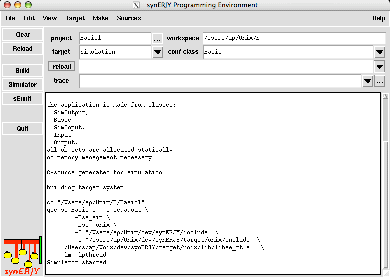
\includegraphics[width=340pt]{../pdf/synerjy-console}
\end{center}
\caption{Screen-shot of the \se\ console}
\end{figure}\label{console-screenshot}

The main text widget displays the command history and the outputs from the
compiler. Most menu entries, display widgets, and buttons should be self-explaining. Note that
buttons are shortcuts for menu entries: \textit{Clear} clears the main
text widget, whereas \textit{Reload} reloads the chosen project after 
resetting the internal compiler database, i.e. all classes from all files 
loaded during the actual session are removed.

\textit{Build} generates code according to the target. The target can be selected as a menu entry. The choice of targets depends on the platform.
Targets may be the simulator (see Section \ref{simulator}) provided by 
the \se\ environment, an executable on the respective
host, or on some micro processor or DSP boards. Target code is executed by 
pressing the \textit{Simulator} button (which is renamed to \textit{Run} in
case of an executable, or to \textit{Upload} if a processor board is the target).

To avoid reloading all files of a project while editing only one file,
the respective file may be chosen in the combobox on the right with 
label \pp{reload} which actually is a button. Pushing the button
reloads the file.

\textit{Quit} terminates the \se\ console.

\subsection{Workspace and Projects}\label{Project}
The \se-environment supports a light-weight project handling. A project consists
of a directory containing a \emph{project resource file} \pp{\_.seprj}.
 The project resource files specifies the 
\se\ files (\pp{.se} files), the \sec\ files (\pp{.sec} files), 
the trace files (\pp{.setr} files), C files (\pp{.setr} files), header files
 (\pp{.h} files), and cclibs (\pp{.lib} files) belonging to a project. 
Files may added and removed using the \emph{project panel} Fig.~\ref{project-panel}. 

The project panel pops up if the entry \textsf{Project} of the \textsf{View}
menu is selected.

\begin{figure}[ht]
\begin{center}
    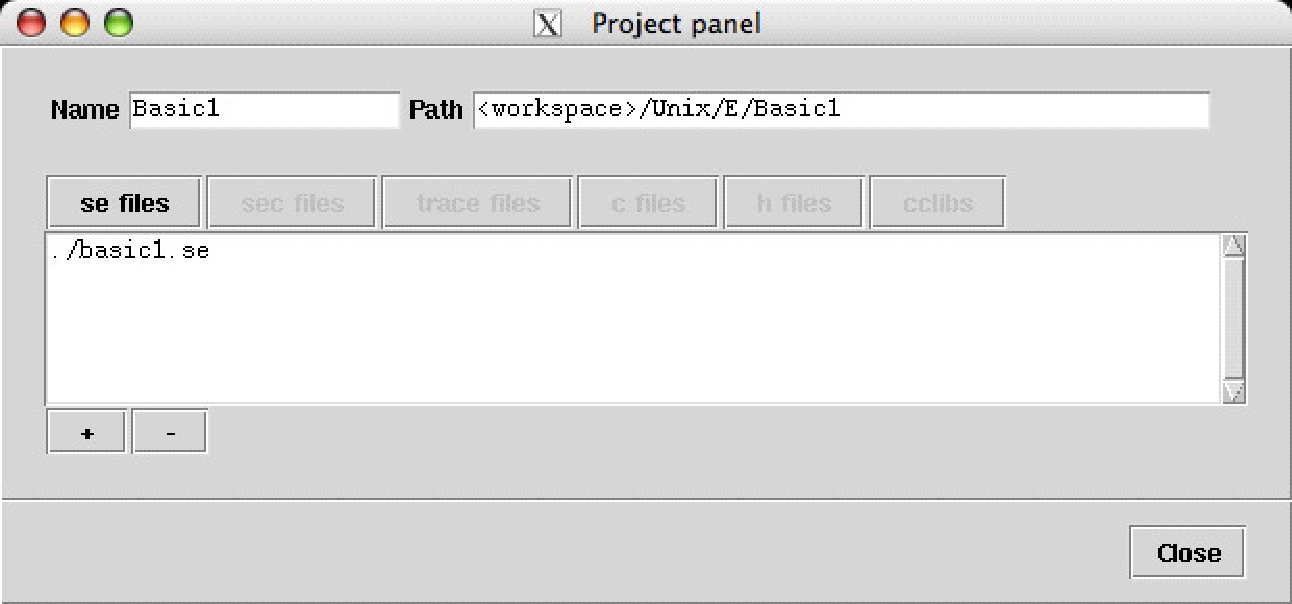
\includegraphics[width=250pt]{../pdf/synerjy-project}
\end{center}
\caption{The synERGY project panel}
\end{figure}\label{project-panel}

All these files have a relative address within \se:
\begin{itemize}
\item relative to a project

\item relative to the \se\ home directory

\item relative to a workspace

\end{itemize}
In Fig.~\ref{project-panel} the file \pp{basic1.se} is defined relative to
the project as indicated by the prefix ``\pp{./}'' (resp. ``\pp{.$\backslash$}'' 
for Windows XP). If the file is addressed relative to the \se\ home directory
the prefix will be ``\pp{<synERJY>/}'', and if relative to the workspace  the
prefix will be ``\pp{<workspace>/}'' (rsp. ``\pp{<synERJY>/}'' and ``\pp{<workspace>/}'' for Windows XP).

A \emph{workspace} is just some other directory which can be chosen using the
preference panel (see Section \ref{preferences}). Default workspace is the
home directory of the respective user. It is required that a project
is a sub-directory of the workspace directory.

The idea of relative addressing is to provide flexibility. Projects may be moved
to an arbitrary position within a workspace if only relative addresses are
used. Similarly \se\ may be installed at an arbitrary place but one may 
still refer to \se\ files provided by the installation. Of course, files may be which are \emph{not} in the project directory, the workspace, the \se\ home 
directory or its sub-directories, but at the price of using absolute addresses, which may make moving and porting projects more difficult.

Projects may be stored or opened, the latter by selecting the entry 
\textsf{Open} of the \textsf{Project} menu (or by double-clicking a project
file in Windows.

A project resource file may be edited. Typical information stored is of the following form:
%
\BEP
// settings for the compiler and the main environment
target Simulation;
set project kind = C-code;
load file = ./basic1.se;
set configuration class = Basic;
load trace file  = ./basic1.setr;
\EEP
%
An overview of all commands is given in Section~\ref{serc}

\subsection{Preferences}\label{preferences}

A few preferences concerning the workspace, and the size and weight of the fonts may be set using the 
\emph{preference panel} (Fig. \ref{preference-panel}).

\begin{figure}[h]
\begin{center}
    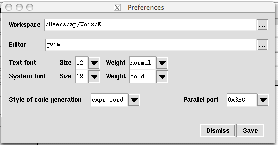
\includegraphics[width=200pt]{../pdf/synerjy-preferences}
\end{center}
\caption{The synERGY preference panel}
\end{figure}\label{preference-panel}
Preferences are stored in as a resource file \pp{.serc} in the \se\ home
directory. All the commands in Section~\ref{serc} may be used within the resource file.

While most of the options are self-explaining, two of them need comments:\begin{itemize}
  \item \se\ allows to generate control code in different styles. The most   
  readable one is \pp{expr-word} where the control structures is given in
   terms a sequential circuit, i.e. Boolean equations representing the logic
   and the control register allocations. In the \pp{expr-bit} each Boolean
   signal or register is coded as a bit in a \pp{char} word. The last style 
   encodes the control structure as a jump table, which is quite an efficient
   implementation for a micro controller.
    
  \item On Windows machines, the parallel port is often used flashing code 
  to micro-controllers. The port name may vary. For convenience some common
  port names are provided to be set using the respective combobox. 
\end{itemize}

\subsection{Environment Variables}
For some applications such as Matlab, Scilab, and the AVR toolset it is 
necessary to set environment variables that should 
refer to the application directories. Environment variables
are set using the menu entries \textsf{Edit$\mapsto$Environment variables}).

\subsection{Building an Application}\label{simTgt}

Often software is built from \se\ classes defined within one file only,
and then is executed in simulation mode. Then it is sufficient to load the
\se\ file, to build the binaries, and to call the simulator.

If the software consists several files including external C functions it usually is
more convenient to define a project.

One should be aware that \se\ compilation usually consists of several steps:
\begin{itemize}

\item Loading of \se\ files builds the internal data structure, type-checks, and
applies semantic checks on class level such as for causality and time races.

\item The building step links the objects, applies semantic checks on the
level of the application, and it generates the executable.

\item The execution step runs the executable on the respective hardware.

\end{itemize}

Since building the executable often implies that first C code is generated, and
then the executable using a cross compiler it is sometimes convenient only
to generate C code. Hence the entry of the \textit{Make} menu.

An experienced user may prefer to use Makefiles. These may be defined using
batch commands as specified in the next section.

\subsection{Commands}\label{serc}

\se\ may be used in ``batch mode'' by using options \pp{se -f <file>} or \pp{se -b <file>} when calling the \se compiler. The file called should consist of a list of
commands. The \pp{-f} starts the interactive GUI after the commands have been executed, 
\pp{-b} terminates after the commands have been processed.

Alternatively, the character \pp{\%} may be used as in
\begin{center}
      \texttt{\small se -b\ \"{}\%set target = atmel;
              load file = can\_test.se; make C-code;\"{}} \\
\end{center}
to treat the \pp{-f} keyword value as commands instead of a file name.
These so-called immediate commands are an easy way to call the \se\ compiler from \pp{make}.

The following settings/commands are supported:

{\footnotesize
\begin{verbatim}
// synERJY - resource and command file

// font used for menu entries and buttons
set system font weight    = normal; // normal and bold supported
set system font size      = 10;     // 8,10,12,14,16,18,20,22,24 supported

// font used for the console window
set font weight           = normal; // normal and bold supported
set font size             = 10;     // 8,10,12,14,16,18,20,22,24 supported

// font used for the simulator windows
set simulator font weight = normal; // normal and bold supported
set simulator font size   = 10;     // 8,10,12,14,16,18,20,22,24 supported

// font used for the graphic editor windows
set graphic font weight   = normal; // normal or bold supported
set graphic font size     = 10;     // 8,10,12,14,16,18,20,22,24 supported

// settings for the graphic editor
set graphic width     = 913;    // approximately a Din A4 page (on my machine)
set graphic height    = 765;    // ...
set graphic file      = name.sc;// default file-name for graphic-editor
set print size        = a5;     // [a4|a5] size for generated postscript

// settings for the compiler and main environment
set load file             = name.se; // for re-load, shown in console window
set configuration class   = Class;   // where main is, shown in console window
set workspace             = /home/user;
                                     // set the workspace
set editor                = gvim;    // editor used if edit invoked from menu
set build                 = make;    // only make supported
clear build;                         // reset build to internal method
target simulation;                   // executable for simulation
target Host;                         // executable for target host computer
target Simulink;                     // executable for Simulink
C-code target             = ...;     // executable for target platform ...
target VerilogSimulation;            // executable for Verilog simulation
Verilog target            = ...;     // executable for Verilog platform ...

set simulation directory  = sim;     // use separate dir for simulation code
clear simulation directory;          // no separate dir for simulation code
set target directory      = tgt;     // use separate dir for target code
clear target directory;              // no separate dir for target code

// commands for the compiler
make binary;                   // generate C-code, compile and link
make C-code;                   // generate C-code only
make build;                    // generate C-code, call make

// load project
set project kind = name.sepr   // load synERJY project
                               // kind = C-code | Verilog

// loading files
set sefile  = mmm.se;          // add synERJY file
set sefile += nnn.swe;         // add further synERJY files
clear sefile;                  // remove all synERJY files

set secfile  = mmm.sec;        // add synERJYcharts file
set secfile += nnn.sec;        // add further synERJYcharts files
clear secfile;                 // remove all synERJYcharts files

set trace file  = mmm.setr;    // add synERJY trace file
set trace file += nnn.setr;    // add further synERJY trace files
clear trace file;              // remove all synERJY trace files

set cfile  = "xxx.c";          // C libraries to add for linking (internal mode)
set cfile += "zzz.c";          // add further libraries
clear cfile;                   // remove all C libraries

set cclib  = "xxx.a yyyy.a";   // C libraries to add for linking (internal mode)
set cclib += "zzz.a";          // add further libraries
clear cclib;                   // remove all C libraries

set vfiles  = "xxx.v";         // Verilog file
set vfiles += "zzz.a";         // add further Verilog files
clear vfiles;                  // remove all Verilog files

clear database;                // ...
clear window;                  // ...
print               = "text";  // print text onto console window

load file           = name.se; // load file
set workspace       = "path"   // set the workspace path
set project path    = "path"   // set the project path

check configuration = Class;   // typecheck application build upon Class

// commands to set the target platform
target simulation;             // target is the build-in simulator
target Host;                   //       ... the host platform
target simulink;               //       ... Simulink
target Makefile;               //       ... as provided by a Makefile in the
                                            workspace directory
C-code target = name;          //       ... the platform denoted by name
target VerilogSim;             //       ... the Verilog simulation environment
   			                                 (using Cver and GTKwave)
Verilog target = name;        //       ... the Verilog platform denoted by name


// Miscellaneous
execute graphic editor;        // ...
execute editor;                // see "set editor=..."
execute file = name;           // read command file name
execute file = "%commands";    // interpret immediate commands
execute file = "!command";     // execute system command (e.g. date)
execute file = "<command";     // read commands from system command (be careful)
set parallel port = "hex"      // set the parallel Port for windows
set code style    = "style"    // set the code style
                               // expr-word, expr-bit,jmp-sty
quit;                          // ...

// commands for the simulator
load configuration file   = name.sim; // load setting (binary,windows) as stored
save configuration file   = name.sim // store setting (binary,windows)
show object browser;                 // ...
show trace browser;                  // ...
show configuration signal = all;     // show all signals (incl. local)

// environment variables
set Matlab directory = path // path of the Matlab directory
set Scilab directory = path // path of the Scilab directory
set AVR directory    = path // path of the AVR directory
\end{verbatim}
}

\subsection{Unit Test}
\se\ programs can be tested using traces. A trace specifies the input 
and output signals at instants, the format of an instant being
%
\BEP
\textit{input$_{1}$} ... \textit{input$_{m}$} -> \textit{ouput$_{1}$} ... \textit{ouput$_{n}$};
\EEP
%
Inputs and outputs are of the form \emph{signal\_name}() for pure signals,
and \emph{signal\_name}(\emph{signal\_value}) for valued signals.

A trace file may be generated using the simulator (cf. \ref{simulator}) or may be
edited by hand. Each trace file consists of one trace.
A trace file generated by the simulator may show additional commands such as 
the command \pp{break} which sets a break point for running the simulator.
Comments are line-wise  starting with \pp{//}.



A unit test may be comprised of several traces. A trace file are either 
loaded using the menu entry  \textsf{File}$\mapsto$\textsf{Load trace file}, 
or by adding it to a project. The latter are stored as part of a project, the
others are temporary: they will be discarded when resetting or closing the console
window.  

A unit test is executed by pressing the button \texttt{sEunit}. The button
is active only if trace files are present. If the test passes
the button flickers in green, if it fails in red. Additionally a message 
is displayed in the console window, e.g. 
\begin{center}
    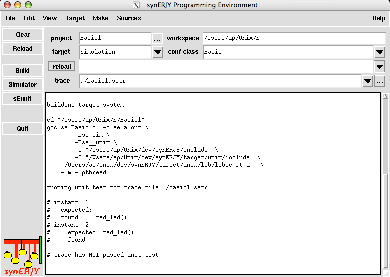
\includegraphics[width=340pt]{../pdf/unit-test}
\end{center}
The message states at what instants conflicts arise between the expected behaviour
and the behaviour found.

In the actual case the \se\ program is 
%
\codeinputuser{basic}
%
with the trace loaded being

%
\BEP
button() -> red\_led();
button() -> ;
-> red\_led();
->;
\EEP
%

\newpage
\section{The \se\ Simulation Environment}\label{simulator}

The simulation environment consists of several components which
allow to trace a programs control flow and
signals. It provides recording and replay facilities for traces.  The
simulator can be started either from the \se\ console( see
Section~\ref{se-console})
or stand-alone, e.g. by typing the shell command {\tt sim}.
 
\subsection{The Simulator Console Window.} 
\paragraph{Introduction.}
The simulator runs as a process on its own.  The simulator
console window is the top-level window for interacting with the simulator.

\begin{center}
    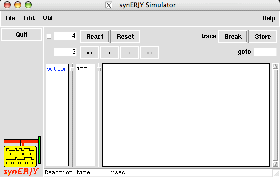
\includegraphics[width=282pt]{../pdf/simulator-console}
\end{center}
The simulator console window allows to step through an \se\ application,
displaying instant by instant. The two main functionalities are:

\begin{itemize}
\item defining the status and values of input signals, and
\item running a program step by step. 
\end{itemize}      

Text widget at the bottom displays system messages such as the reaction
time which is the time used by the simulated \se\ program (not including
the time needed for simulation). Execution time, of course, depend on
the target machine, hence the reaction time shown specifies the time used
if the program is run on the same machine that executes the simulation.
It has little bearing for other target machines, except that the ration
of reaction times for different instants indicates which computations
might be costly.

\paragraph{Defining the status and values of input signals.}
The input widget
\begin{center}
  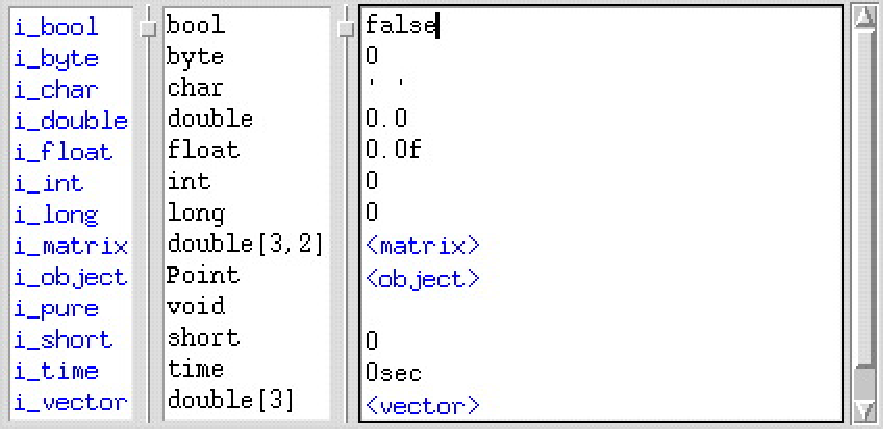
\includegraphics[width=230pt]{../pdf/input-widget}
\end{center}
of the simulator console window three subwidgets: 
\begin{itemize}
\item the left  widget displays the signal names and indicates by colour
      whether a signal is present or absent. They are displayed in
      blue if absent and in red if present.  The user can
      determine their status via the left mouse button.  A
      simple click on a signal name toggles presence and absence
      (red and blue).  The signal will be present for only one
      instant.  A click with additionally the shift button
      pressed will turn a signal name green; this means that
      presence will persist.  A simple click will turn the
      green to red.
      
      The signal value used for the next presence of the signal must be
      typed into a text widget. Hitting the return key sets the signal to 
      present while checking whether the corresponding values are 
      well-formed. Alternatively, the signal can be set present using
      the toggle described above, also checking the well-formedness of
      values.
      
      In case of errors direct feedback is given in the entry line
      on the bottom of the widgets

      \item the middle widget displays the signal types.

      \item the right widget displays the signal values.  It is a
      restricted text widget for specifying the values.  If the return
      key is hit, the values are checked for being well formed and the
      respective signal is set to red.  Errors will be
      indicated in the error message entry at the bottom of the
      simulator console window.
\end{itemize}

For structured values such as vectors, matrices, or objects only the kind
is indicated as active text. Clicking on the signal name opens an input
panel such as
\begin{center}
  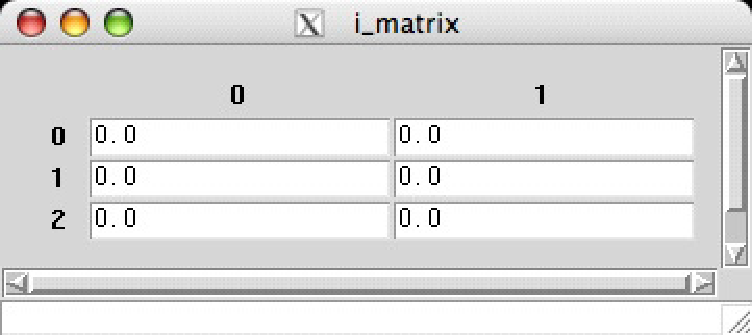
\includegraphics[width=230pt]{../pdf/matrix-widget}
\end{center}
Values can be set as suggested above for simple signals.

\paragraph{Running the Simulator in Single Step Mode.}
The upper widgets of the simulator console window
\begin{center}
  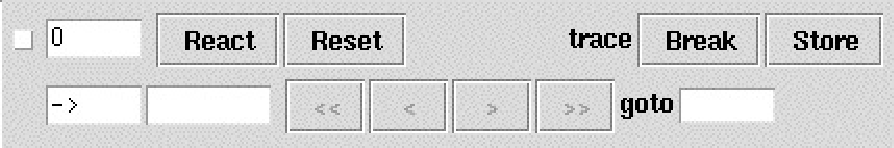
\includegraphics[width=230pt]{../pdf/run-widget}
\end{center}
consists of several buttons: 
\begin{itemize}
    \item The \textsf{React} button causes execution of a single step.
    \item The \textsf{Reset} button resets the simulator. 
\end{itemize}
These are the main actions for driving the simulator.  One might step
backward and forward through the instants already executed by the
following buttons:
\begin{quote}
    \begin{itemize}
    \item Button \texttt{<}  : one instant backward 
    \item Button \texttt{>}  : one instant forward 
    \item Button \texttt{<<} : to the very first instant 
    \item Button \texttt{>>} : to the very last instant 
    \end{itemize}
\end{quote}
Inserting a positive integer in the \texttt{goto} widget, and hitting the
return key, brings you to the respective instant.

\paragraph{Terminology.}
We distinguish between three kinds of instants:
\begin{itemize}
    \item the \emph{next instant}: the next instant to be
    executed.  The number of the present instant is shown in the box
    in the upper left corner.

    \item the \emph{previous instant}: the last instant executed. 

    \item the \emph{displayed instant}: the instant that has been chosen by
    stepping backwards or forwards or by using the goto widget.  The number of
    the respective instant is shown below. Just after a reaction the number of
    the previous instant is displayed.

\end{itemize}

There are two more buttons for recording traces. 
\begin{itemize}
    \item The \textsf{Break} button sets a break in the
    trace.  The button is a toggle
    \texttt{Break}$\leftrightarrow$\texttt{Unset}:
    if a break is set it may be unset.

    \item The \textsf{Store} button stores the present trace into a file.
\end{itemize}

Traces are stored for a replay: the stored sequence of the signals presences and
their values can be extracted automatically from a file and used as input for
another test run. Replaying is initiated from the
\textsf{Utils}$\mapsto$\textsf{Open trace file} menu entry. An opened trace
file will result in a slightly modified simulator console window.
\begin{center} 
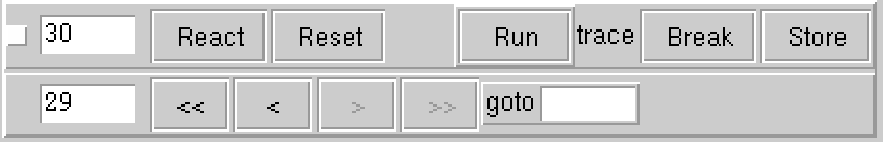
\includegraphics[width=230pt]{../pdf/simulator-replay}
\end{center}

The small box on the left of the simulator console window
turns to red. The additional button 
 \begin{itemize}
     \item The \textsf{Run} button executes all of the activated
     trace files up to the next break (the end of
     a trace file defines a break by default).
 \end{itemize} 

\subsection{The Object Browser.}

The object browser is the main interface for organising the configuration of
the \se\ simulator.  It displays the object hierarchy. A "\textsf{+}" in front of
an object name indicates that there are sub-objects to the respective object.
Clicking with the left mouse on "\textsf{+}" opens the hierarchy which can be
closed again by clicking on "\textsf{-}". For each object, a \emph{pop-up menu}
is displayed when clicking the left mouse button on its name.  
There are three entries:

\begin{itemize}
\item \textbf{Show Class} displays the respective class.
      
\item \textbf{Show Animation} opens the animator for the respective object.
      
\item \textbf{Show Traces} calls the Trace Browser that displays the trace
      of the signals and attributes of the respective object.
\end{itemize}
    
\subsection{The Animator.}\label{animator}
The animator highlights the halting points and the emitted signals of the reactive 
code. Selecting ``Show Animation'' opens a text window displaying the constructor 
of the respective object.
    \begin{center}
        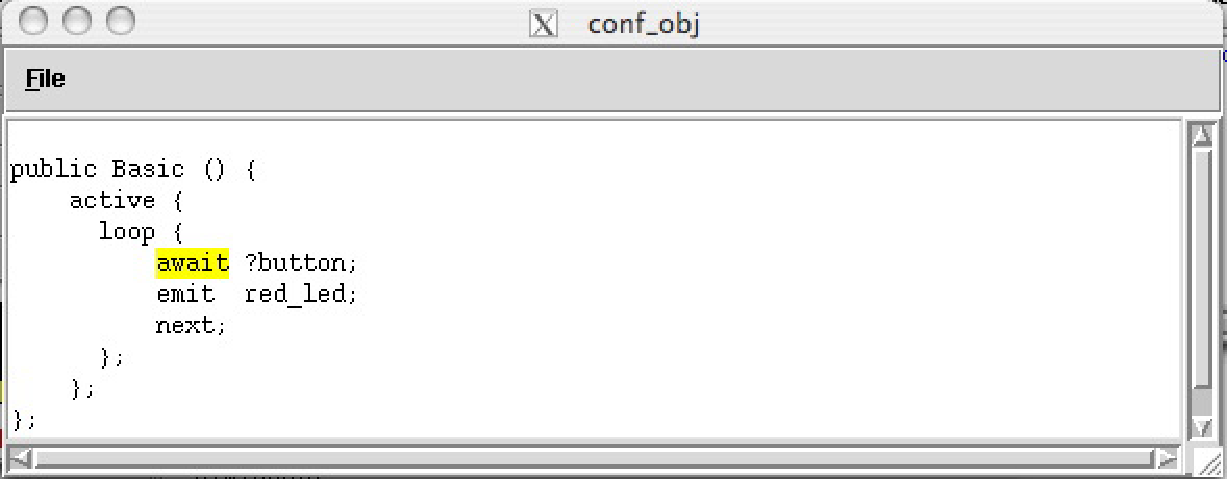
\includegraphics[width=260pt]{../pdf/confobj1}
    \end{center}
The halting points are marked by a yellow background, the signals emitted by a 
light-blue background.
    \begin{center}
        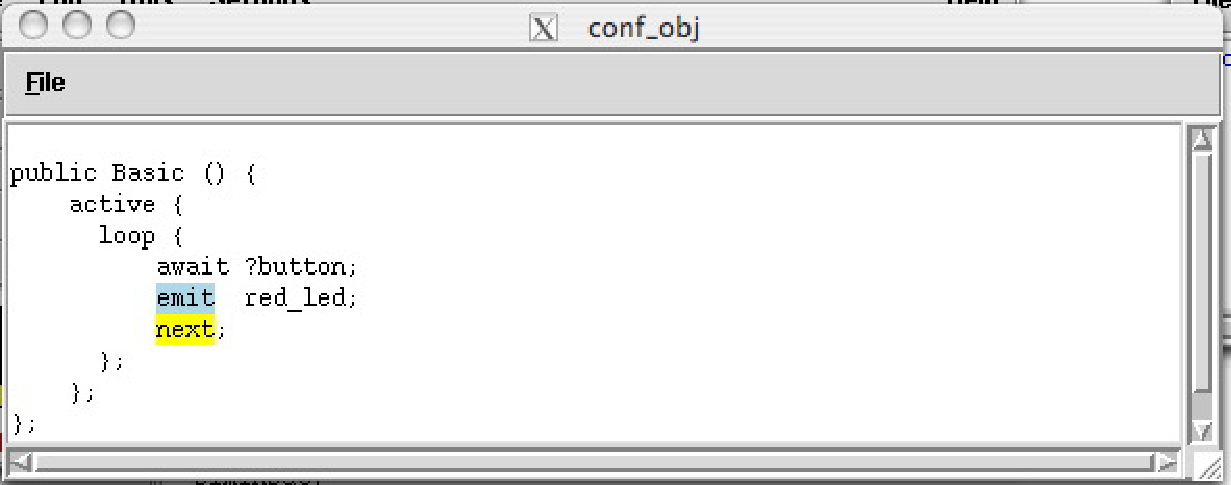
\includegraphics[width=260pt]{../pdf/confobj2}
    \end{center}
Within such code there may be references to reactive reactive or graphical
presentations of automata. These are indicated by a blue foreground as in 
    \begin{center}
        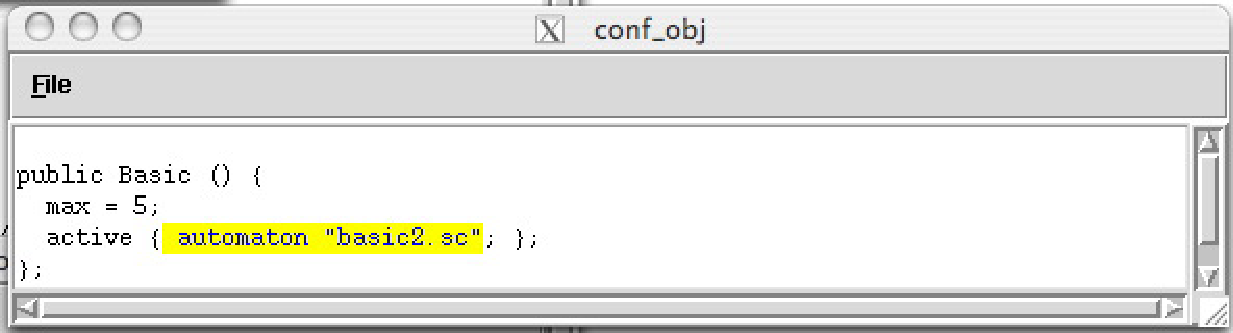
\includegraphics[width=260pt]{../pdf/confobj3}
    \end{center}
The yellow background specifies that the automaton is active. The active state
in such an automaton is highlighted in orange while the transition taken again 
is highlighted in blue as in
    \begin{center}
        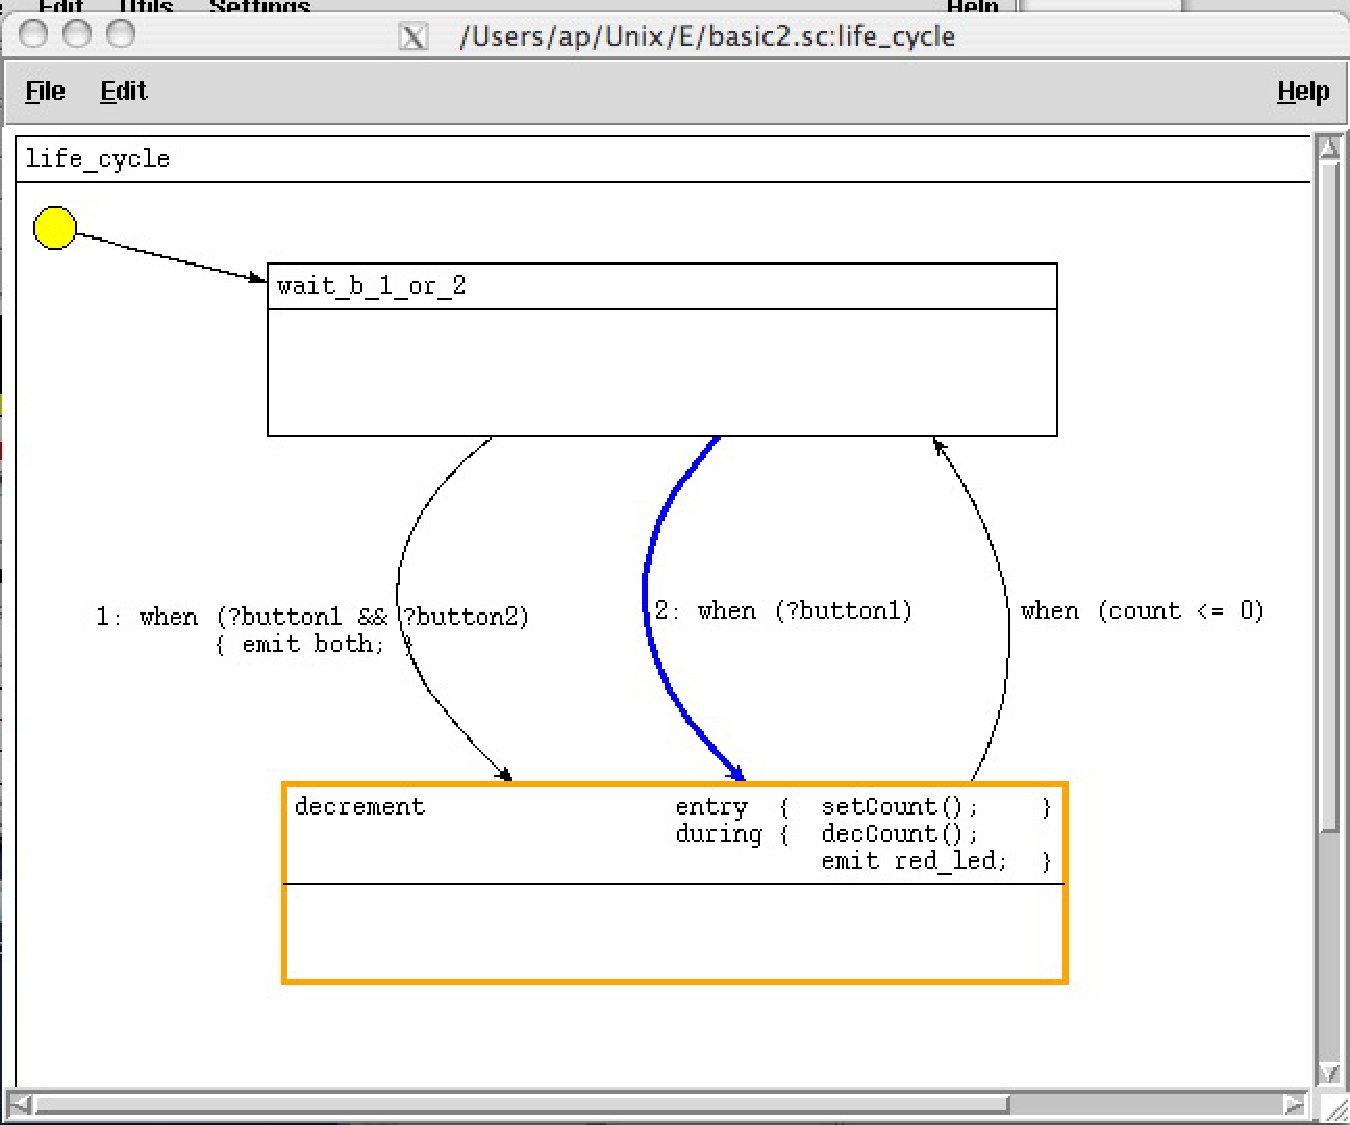
\includegraphics[width=260pt]{../pdf/automaton}
    \end{center}

\subsection{The Trace Browser.}\label{trace-browser}

The trace browser displays the status and the value of all the signals
of an object, and the values of all attributes.
\begin{quote}
    \begin{center}
        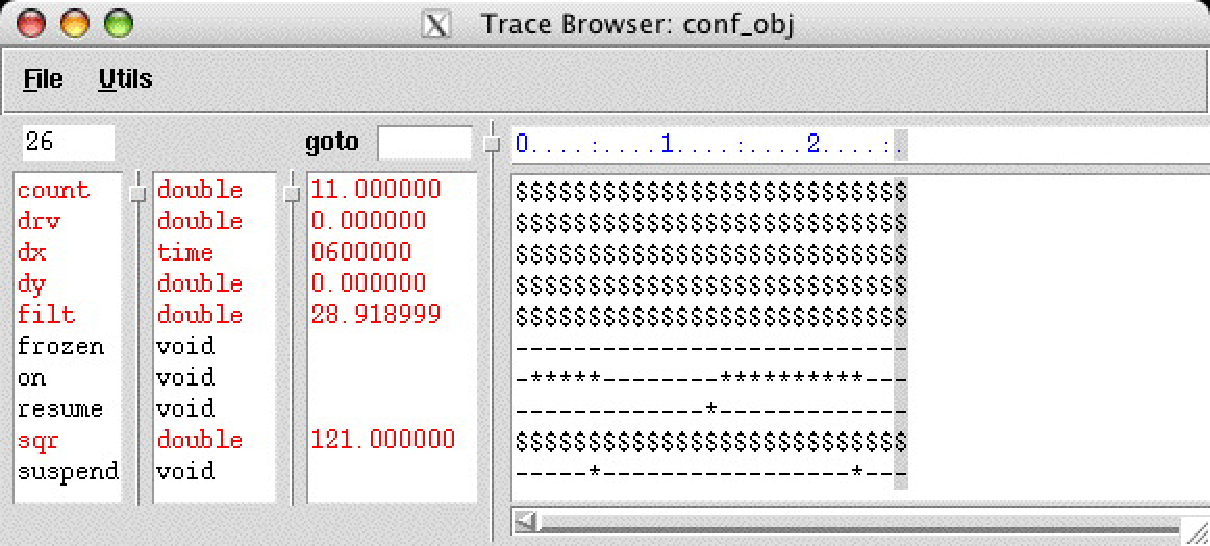
\includegraphics[width=260pt]{../pdf/trace}
    \end{center}

    The panel displays from the left: 

    \begin{itemize}
    \item \emph{name}: A signal is highlighted in
    red if it is present at the displayed instant (the displayed
    instant is indicated in the upper left widget)
 
    \item \emph{type}
    \item \emph{value}

    \item \emph{instant number}: the small window indicates by special
    characters and numbers the instants displayed (modulo 100). By clicking
    with left mouse button, the instant displayed under the mouse cursor
    becomes the displayed instant. By marking a region of instants (by clicking
    and dragging the left mouse button), all the values of this region will be
    displayed in a separate window, a so called \emph{Value Sample
    Panel} (see below).

    \item The \textit{field traces}.
     The lower right large widget indicates absence of a signal ba a ``-''.
     Presence of a pure signal is indicated by
     "\*", and that of a valued signal by by ``\$''.
     For Boolean-valued signals we use ``t'' and false to indicate the value
     in case that the signal is present. 
      The highlighted bar indicates the displayed instant.
    \end{itemize}
\end{quote}       

Inserting a positive integer in the goto widget, and hitting the
return key, moves to the respective instant.

\subsection{The replay panel}
allows to organise the replay of trace files. 
Several trace files may be active.  Trace files are (de-) activated or
deleted using a pop-up menu.  The menu is opened by clicking the left
button with the cursor being over the file name.

\begin{center}
    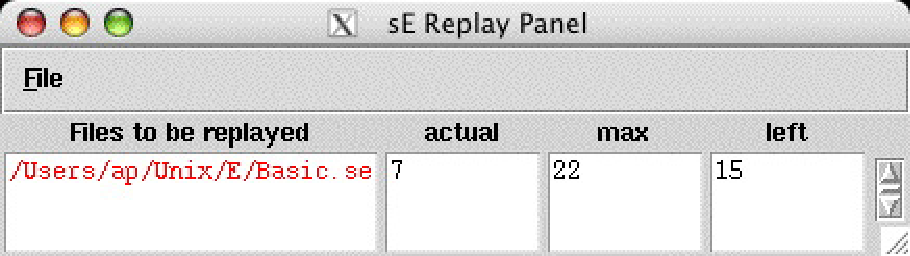
\includegraphics[width=270pt]{../pdf/replay-panel}
\end{center}

\subsection{The Signal Choice Panel}
The signal choice panel allows to change the set of signals and 
attributes displayed by a trace browser.

\begin{center}
    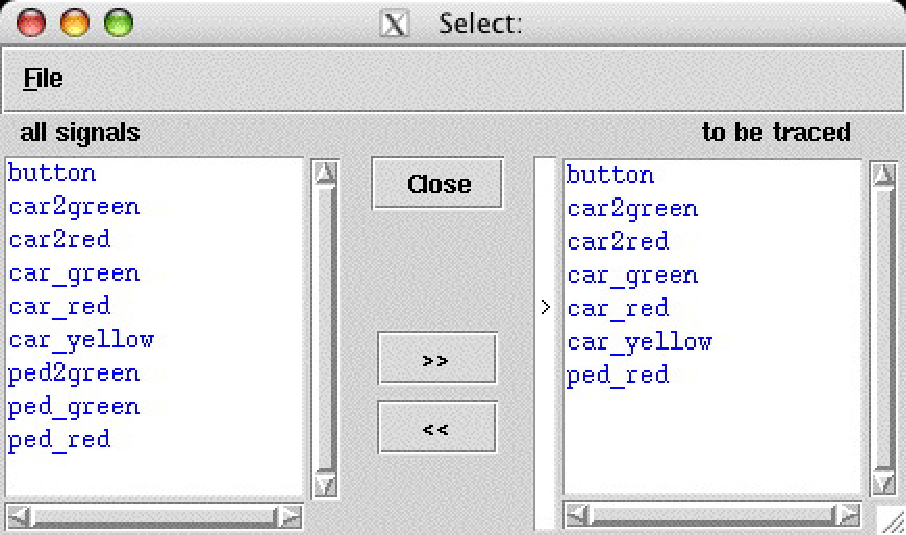
\includegraphics[width=220pt]{../pdf/select-panel}
\end{center}

Marking a sequence of signals with the mouse on the right hand side
and pushing the button \texttt{<<} eliminates
the signals and attributes.  Marking on the left hand side and pushing
the button \texttt{>>} adds starting from
the position indicated by the marker \texttt{>}.

The marker \texttt{>} can be changed by clicking on the intended position
in its widget.

\subsection{The Value Sample Panel}
displays all the values of signals in a specified
region of instants.  It is opened from the trace browser.
The highlighting indicates the displayed instant.
\begin{center}
    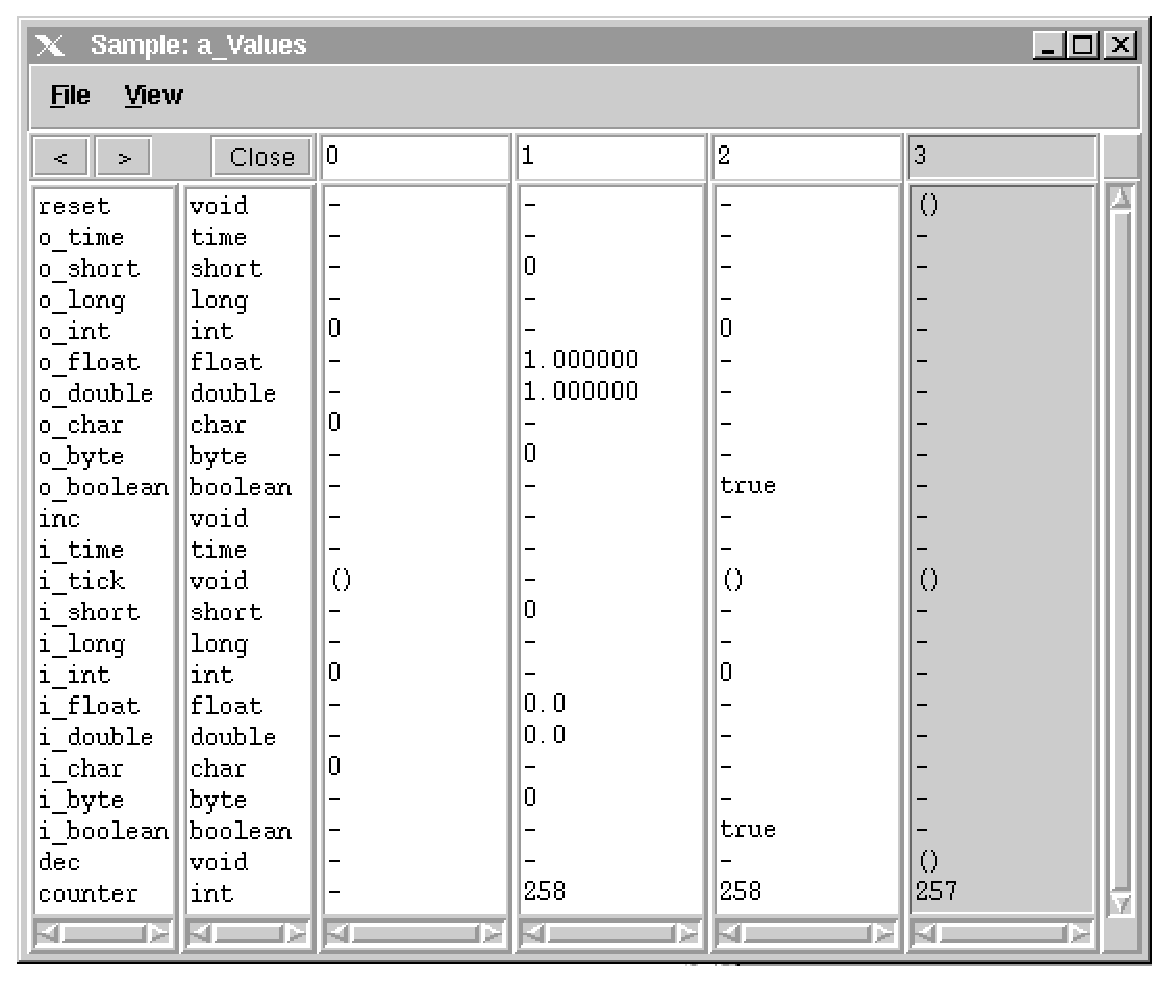
\includegraphics[width=270pt]{../pdf/matrix}
\end{center}
The window behaves like a sliding window: by pushing the
buttons \texttt{<} and \texttt{>} the displayed region
moves forward or backward.

\subsection{Error panel}
An error panel pops up in case of some error.

\newpage
\section{\emph{synERJYcharts} - The Graphic Editor}\label{graphic-editor}

\se charts are graphical presentations of hierarchical state machine. These can
be visualised and edited using the graphical editor. \se charts are
stored in a binary format in files, suffixed with \pp{.sec}.

The graphic editor for \se charts may be started 
\begin{itemize}
\item from the \se\ console window,
\item by typing the command {\tt ge} in a shell (for Unix systems only), or
\item by double clicking the icon of a \pp{.sec} file  (for Windows only).
\end{itemize}

\subsection{The Graphic Editor Console Window}
The graphic editor console window
displays the hierarchy of states if a graphics file is loaded.
\begin{center}
    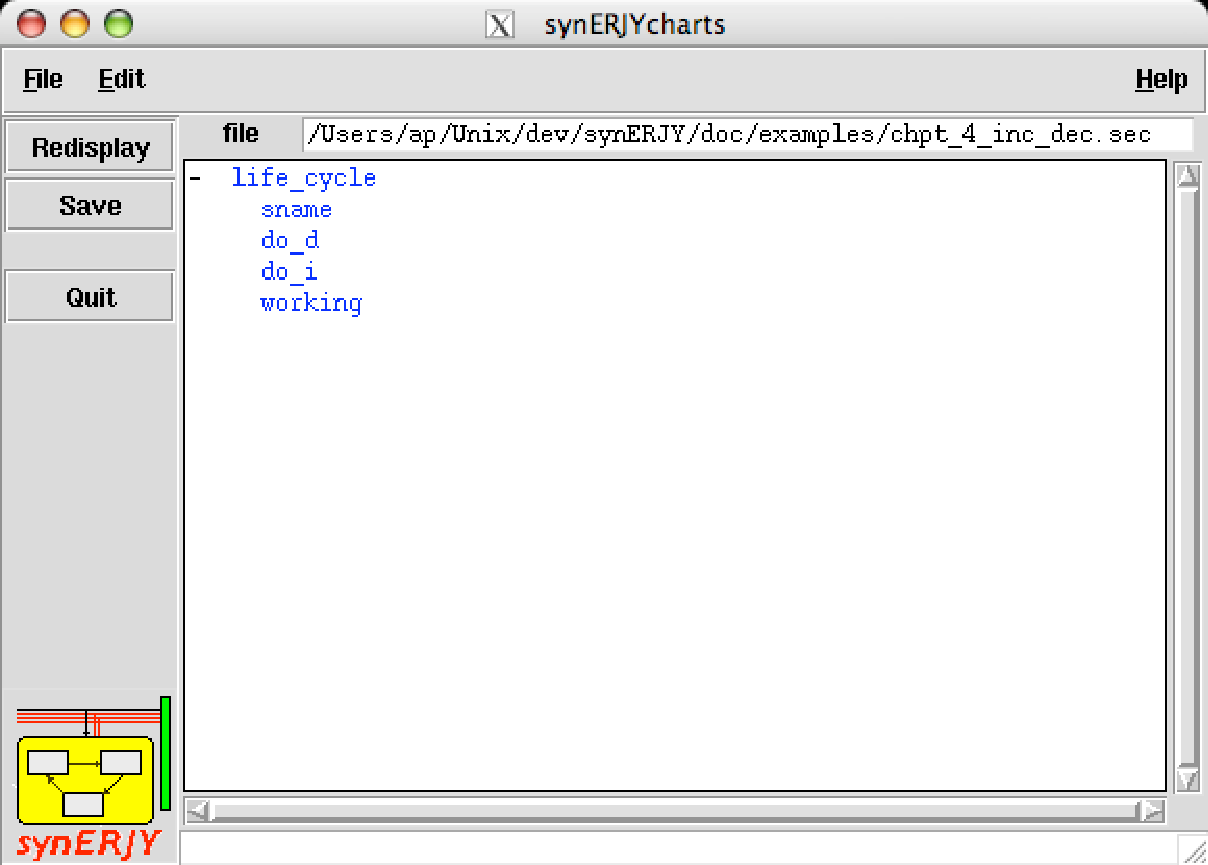
\includegraphics[width=220pt]{../pdf/ge-console}
\end{center}

\subsection{The Graphic Editing Window}
\paragraph{Editing a graphic.}
A graphic consists of graphic objects such as states, transitions,
initial nodes and conditional nodes.  For each kind,
there is a specific tool to create and manipulate a graphic object. 
Editing takes place in a graphic edit window.
\begin{center}
    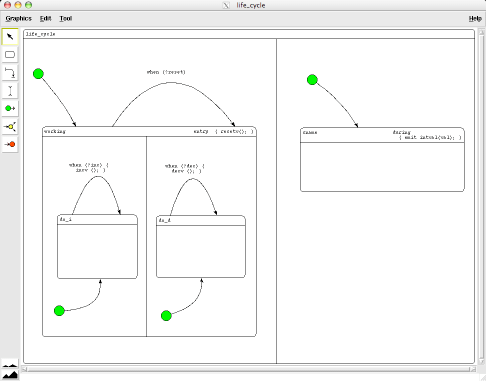
\includegraphics[width=340pt]{../pdf/ge-window}
\end{center}

The main widget is the drawing widget. On the left there are the tool 
button. The entry line at the bottom is an \emph{info window}. It 
displays information as well as error messages.

All graphic objects in a window have a number, the ``graphic object id''.
Entering a number in the info window and hitting
the return key, highlights the respective object. Note, that
\emph{error messages} of the \se\ Console may refer to graphic object
id's.

%\paragraph{Mouse and cursor.} The graphic editor uses the left
%mouse button (B1) to select tools, or existing graphical
%objects, or existing text, and to position new graphical objects 
%on a graphic-window. Using the modifier Shift, further graphical 
%objects may be added to the selection. If an item, or group of items, is selected, B1 is used to move these. Double clicking B1 on a text opens a window for text editing. double clicking on a state opens a new 
%graphic window referred to as \emph{refinement} of a state.

%The image of the cursor is changed for visual feedback.

\paragraph{Tools.} The tools create and modify graphic objects on
 the drawing widget.
\begin{itemize}
\item[] 
\includegraphics[width=20pt]{../pdf/point-tool}\hspace{10pt}
\textit{Point Tool}: select, move, and resize graphic objects.

\item[] 
\includegraphics[width=20pt]{../pdf/state-tool}\hspace{10pt}
The {\em State Tool}: create persistent states.

\item[] 
\includegraphics[width=20pt]{../pdf/transition-tool}\hspace{10pt}
 {\em Transition Tool}: create transitions.

\item[] 
\includegraphics[width=20pt]{../pdf/and-tool}\hspace{10pt}
 {\em And Tool}; create new and-states for a selected (super-) state.

\item[] 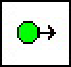
\includegraphics[width=20pt]{../pdf/init-tool}\hspace{10pt}
{\em Init Tool}: create initial transient states.

\item[] 
\includegraphics[width=20pt]{../pdf/condition-tool}\hspace{10pt}
 {\em Condition Tool}: create conditional transient states.

\item[] 
\includegraphics[width=20pt]{../pdf/exit-tool}\hspace{10pt}
 {\em Exit Tool}: creates termina transient states.

\end{itemize}

\PP{Creation.} Graphic objects are created by pressing the left mouse button B1,
moving, and releasing it. Moving determines the size.
 For transitions, the cursor must be on a state (source
state) before pressing B1. Dragging the cursor to the target state and
releasing B1 will create a transition.  Some constraints are checked for
minimal sizes of state-boxes or minimal distances of transitions to edges of
state-boxes, etc.  Remarks and errors are reported in the info-window.\\

\PP{Selection.} A single or a group of graphic objects is selected either by
clicking B1 on an object or by clicking B1 on the graphic window and then
dragging with B1.  All graphic objects contained in the rectangle spread by the
dragging are selected.  Adding to a selection is done by pressing the Shift-key
and clicking B1.

Selection of graphic objects generates handles for manipulating the object.  In
case of transitions, the red handles refer to the arrow of the transition, the
yellow handle refers to its label.\\
  
\PP{Moving.} A single or a group of graphic objects may be moved only after
selecting them.  B1 is pressed, moved towards the desired direction of the move
and then released.  Visual feedback is only given after B1 is released.
Repeat if you want to improve the move.\\

\PP{Resizing.} Resizing is possible only if a single graphic object is
selected.  B1 is pressed very close to one of the
handles of the graphic object and released at the desired place.  Visual
feedback is only given after B1 is released. Repeat
to improve the resize.

If a transition is resized, the source and target handle, the side of the
state-box to which it is attached, the bending of the transition and the
placement of the label may be modified.\\

\PP{Editing text.} All text in the graphics can be edited.  Double click B1 on the text. The \emph{Text Edit Window} will be opened.
\begin{center}
    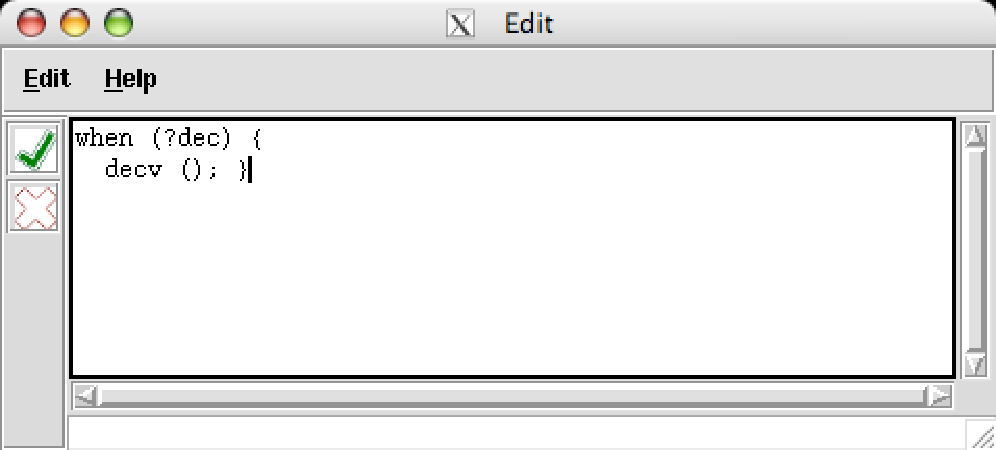
\includegraphics[width=230pt]{../pdf/ge-text-window}
\end{center}
This simple text editor can be used
for changes.  Pressing the {\em Accept} button checks whether the 
text is syntactically correct according to its
position.  If accepted the text is copied to the graphics, otherwise
an error message is displayed in the the line below the text widget. 
If the Text Edit Window is closed by pressing the button \emph{Reject}
the old text is kept in the graphics.\\

\PP{Refining a state.} Any state may have sub-states (If the state has
sub-states, it is called a super-state). Few sub-states including their
transitions may be put into the box indicating the place of the super-state. If
a super-state has many sub-states, it is recommended to put them into a
separate window, the \emph{refinement window}. Double clicking on a state opens the refinement window. This window contains the complete substructure of the super-state (often called the and-or-decomposition). The refinement may be 
cancelled using the \pp{File->Undo refinement} in a refinement window. But
note that all existing substates in the refined window will be lost.

\PP{Actions.} There are several action which may be defined textually in a state.
\begin{description}
\item[\pp{entry \{\emph{action}\}}] - an instantaneous action executed when entering a state.
\item[\pp{exit \{\emph{action}\}}] - an instantaneous action executed when exiting a state.
\item[\pp{during \{\emph{action}\}}] - an instantaneous action which is executed  while being in a state.
\item[\pp{do \{\emph{action}\}}] - an action the execution of which starts when entering a state, and terminates when exiting a state.
\end{description}
The action are specified in the right upper corner of a state box, e.g.
\begin{center}
    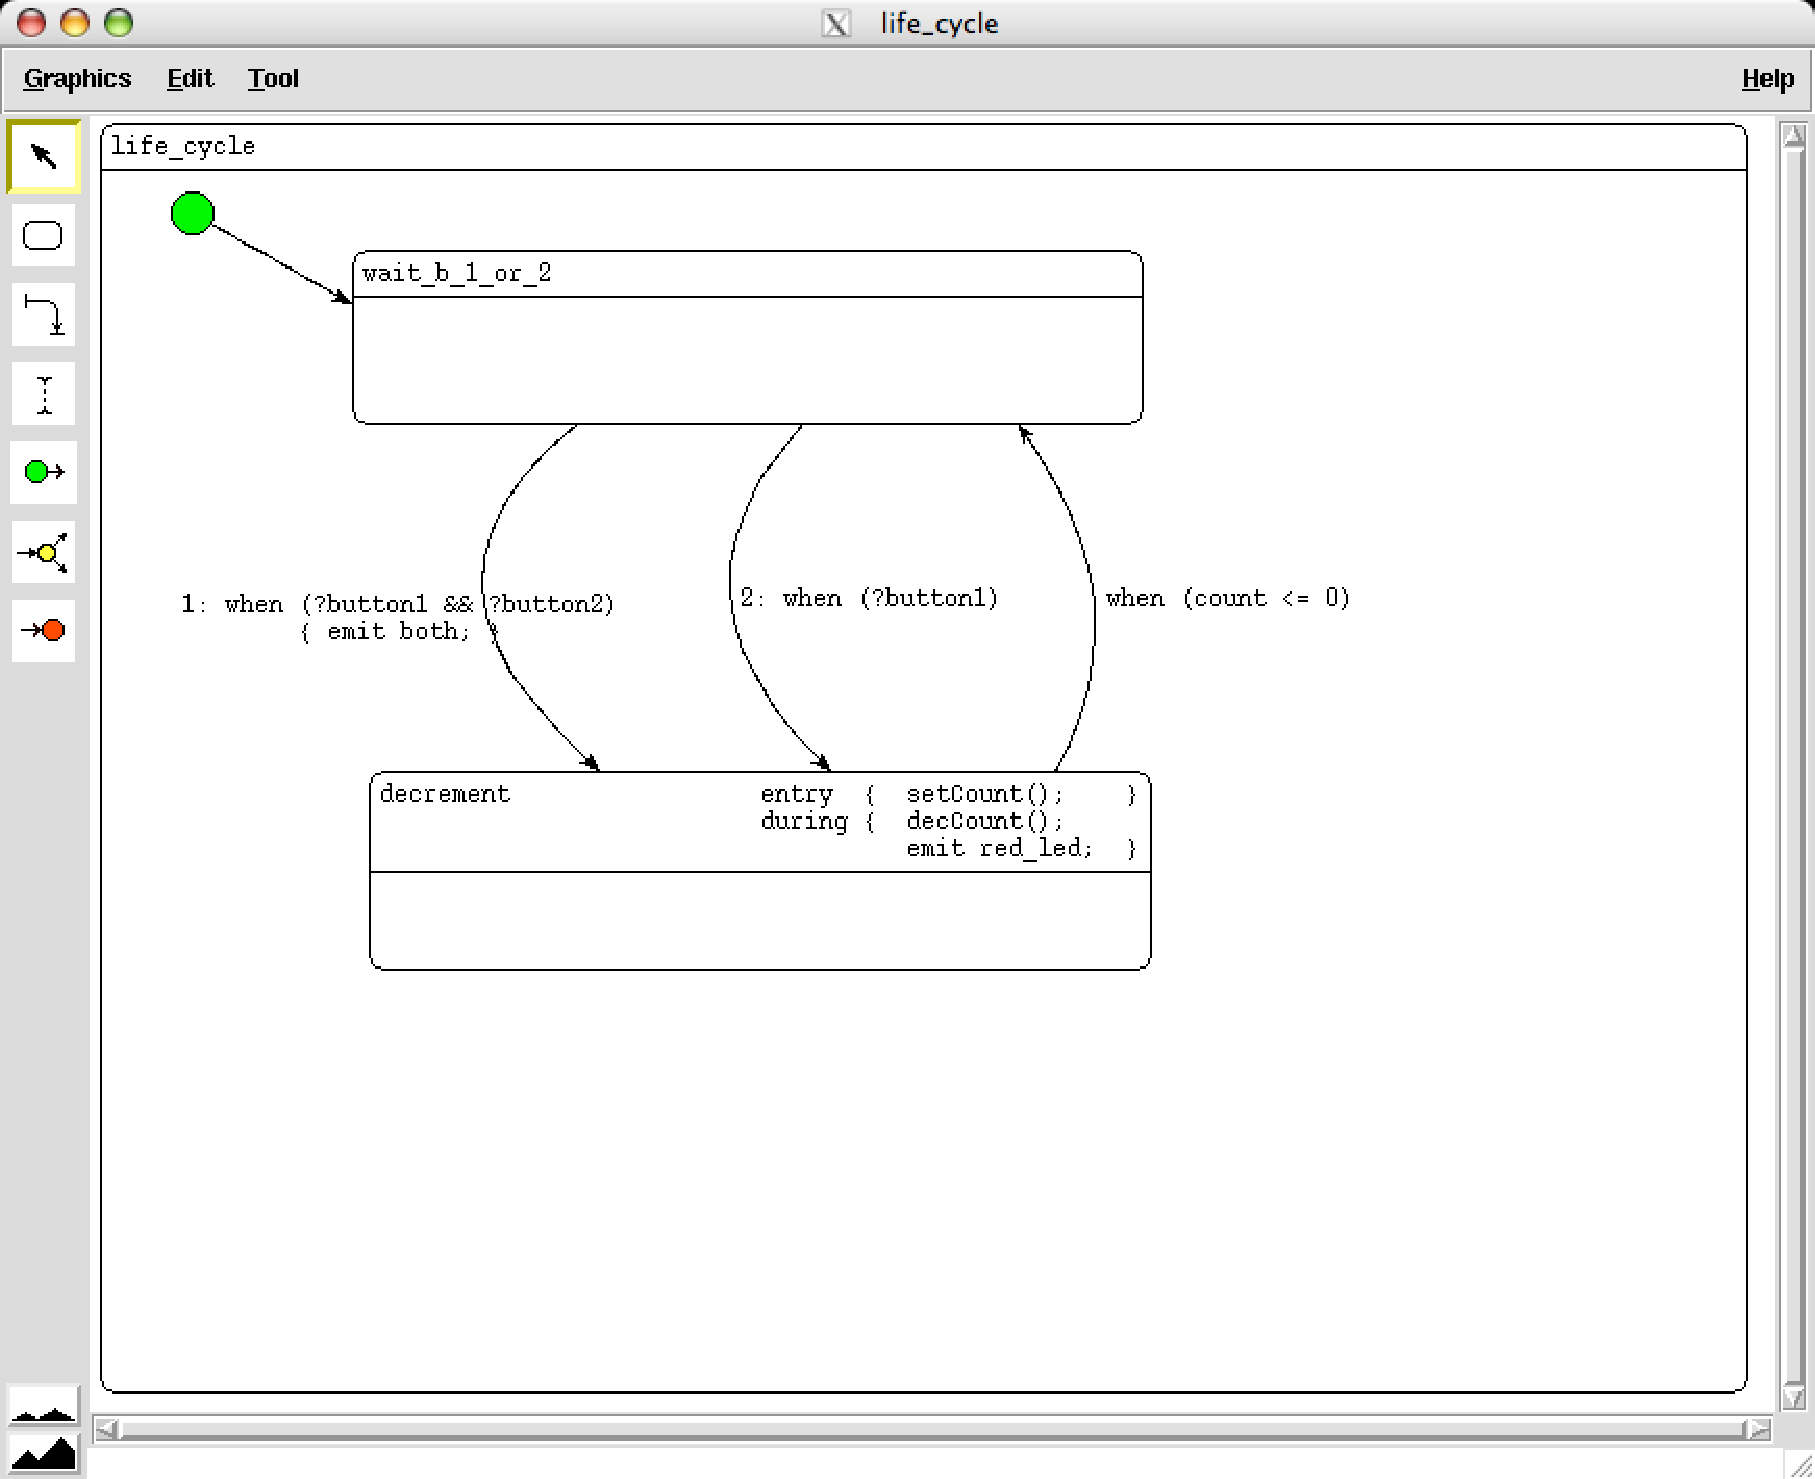
\includegraphics[width=300pt]{../pdf/action-example}
\end{center}

\PP{Textual states.} Sometimes the it is convenient to consider states with textual actions being exclusive. In that case the perspective may be switched
in that the actions are displayed beneath the separating line, e.g.
\begin{center}
    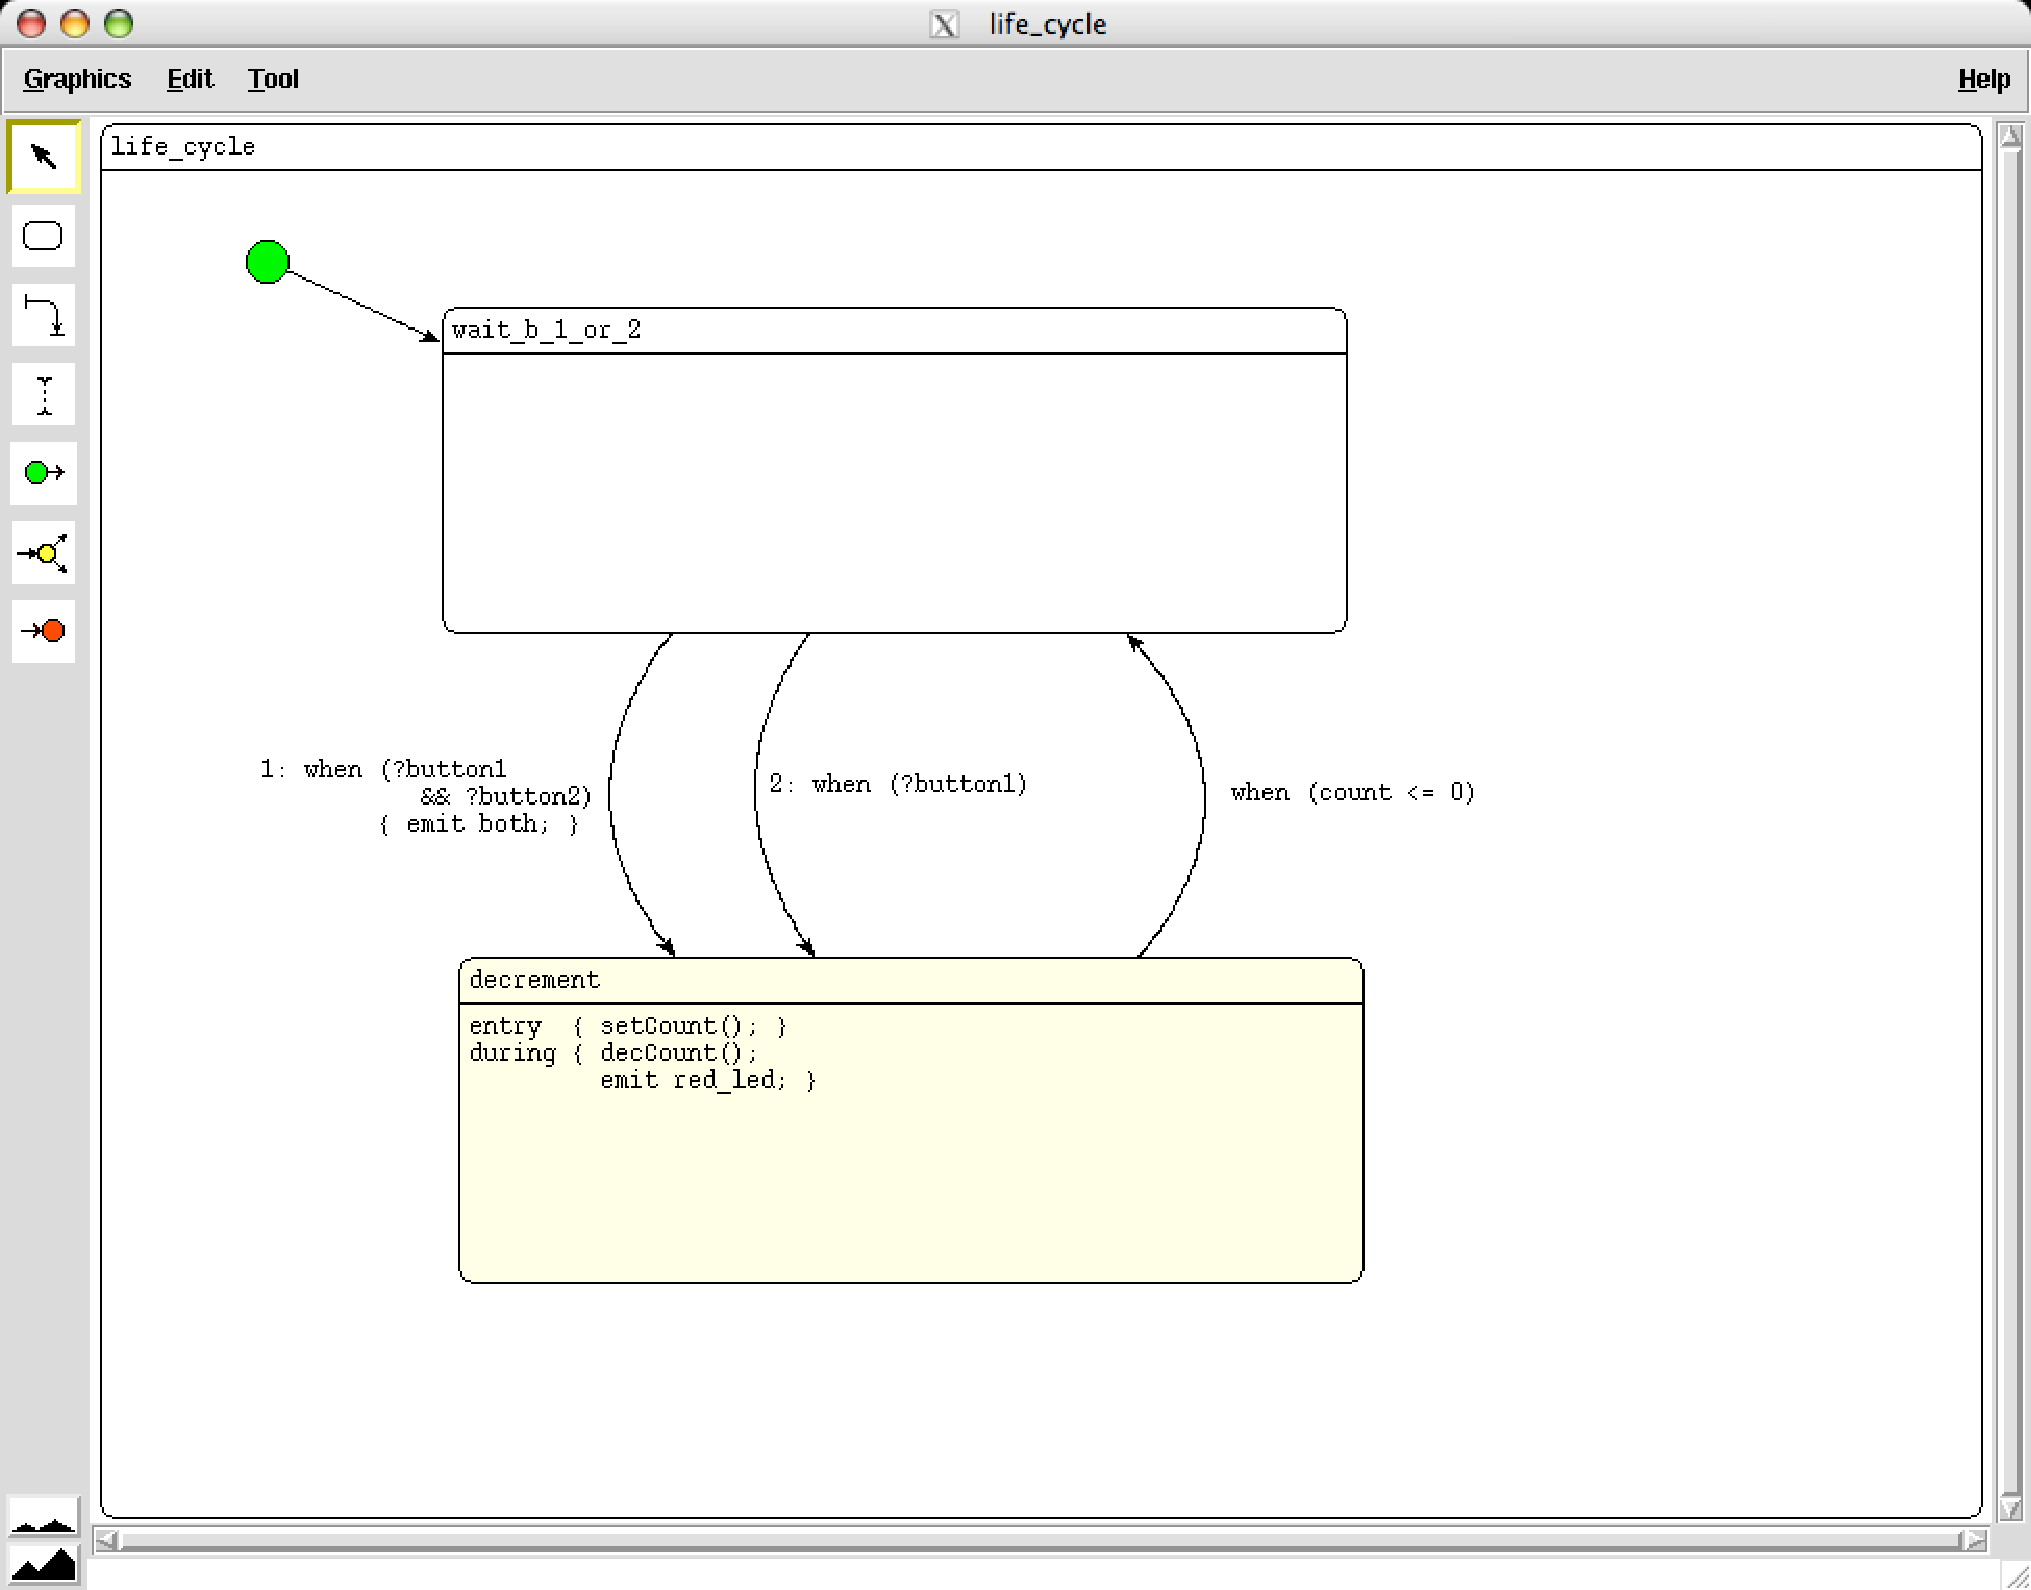
\includegraphics[width=300pt]{../pdf/action-example-2}
\end{center}
The switch is achieved using a the context menu for state actions (see below).

\PP{Context menus.} Clicking the right mouse button opens several context menus. Click on the
\begin{description}
\item[\textbf{canvas}] - to switch the tool, or to paste a state
\item[\textbf{state name}] - to change the font size and weight
\item[\textbf{state action}] - to change the font  size and weight, or the switch to a textual state
\item[\textbf{transition text}] - to change the font  size and weight
\end{description}

For instance, there is a context menu 
\paragraph{Known problems.}
\begin{itemize}
\item Attaching transitions to state-boxes is not too smooth. This may sometimes be irritating in particular for small state boxes.

\item Reducing the size of a state-box is rejected if the transitions attached become disconnected.  The rule to detect this, however, is sometimes obscure. To
overcome this problem, you may attach transitions temporarily to other states,
resize the state, and re-attach the transitions.

\end{itemize}

\newpage
\section{Model-based Design}

\subsection{An Upshot of Model-based Design}
Model-based design distinguishes between the environment (or plant) and the controller that is embedded into the environment. Both environment 
and and controller may range from being simulation software 
to the real hardware on the environment side and embedded controllers
on the controller side.

The typical design cycle proceeds in several steps:
\begin{description}
  \item[Model-in-the-Loop] Both environment and controller are coded in 
          a simulation tool, for instance in Matlab/Simulink \cite{Matlab} or
          Scilab/Scicos \cite{Scilab}.
  \item[Software-in-the-Loop] The controller is replaced by a binary (e.g.
          an Sfunction in case of Simulink, or a new block in case of Scicos). 
  \item[Virtual-Silicon-in-the-Loop]
          The controller runs on an instruction set simulator that interacts
           with the simulation environment.
  \item[Processor-in-the-Loop]
          The controller runs on the target hardware  that interacts
           with the simulation environment.
  \item[Rapid Prototyping]
          The controller runs on a PC/workstation  that interacts
           with the real environment.          
  \item[Rapid Prototyping on Target System]
          The controller now runs prototypical ECU.   
  \item[Hardware-in-the-Loop]
          The controller runs on a production ECU but in a HIL system.
  \item[Final Product]
          The controller now runs production ECU.   
   \end{description}
\se\ supports Software-in-the-Loop in that it generates executables for
 Matlab's Simulink and Scilab's Scicos. The same code (minus instrumentation)
 may run on the supported hardware emulators or target hardware.
 
\subsection{Generating Sfunctions for Simulink.}
\se\ programs are integrated in Simulink diagrams using Sfunctions: 
for building an Sfunction 
\begin{itemize}
\item the target must be set to Simulink
in the \se\ console (\textsf{Target$\mapsto$Simulink}).
\item the environment variable for the Matlab directory must be set
using the \emph{environment variable panel} 
(\textsf{Edit$\mapsto$Environment variables}).
\end{itemize}
 The name of the generated Sfunction is that of the configuration class. 

To use this Sfunction in a Simulink diagram, insert an Sfunction block,
\begin{center}
    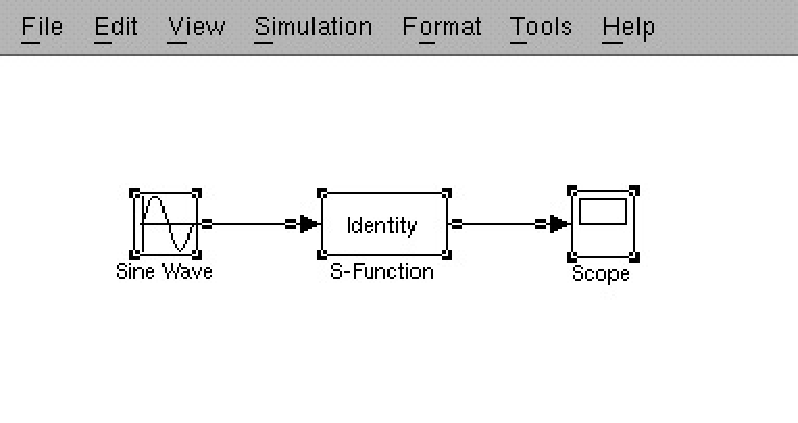
\includegraphics[width=180pt]{../pdf/Simulink-1}
\end{center}open its property list, and enter the name
of the configuration class. 
\begin{center}
    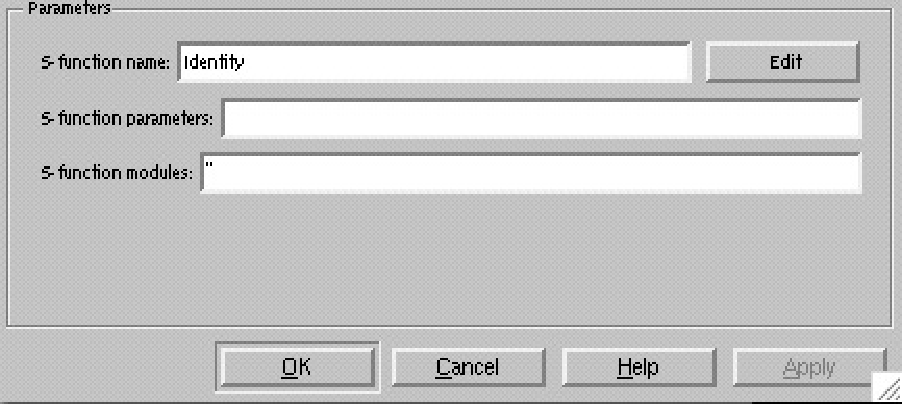
\includegraphics[width=150pt]{../pdf/Simulink-2}
\end{center}
For proper 
operation it is recommended to start Simulink from within the respective 
\se\ project directory.

\emph{Parameters} are supported. Parameters may be of all the types supported by
Simulink. Type constraints may be needed: e.g. \pp{0} will not automatically
considered as being an integer, but one needs to specify its type, for instance
\pp{int32(0)} to be of \se\ type \pp{int}.

The \emph{timing constant} \pp{timing} determines sampling time of the Sfunction 
block. If the timing constant equals \pp{0sec} the sampling time of the
block will be inherited by the environment.

\emph{Exceptions} are raised by \se\ will be shown as Simulink exceptions.

\emph{Feedtroughs}, i.e. signals the output of which at an instant depends on
the input of some sensor at the very same instant, are detected and flagged
as such, hence may give rise to ``algebraic loops''. 

\paragraph{\textit{\textbf{Warnings}}} 

\begin{itemize}
  \item The method main is ignored when a 
  SIMULINK S-Function is generated. Inspect the method body to check 
  whether this may cause problems (often initialisation code can be moved to
  the constructor of the configuration class).
  \item On Windows, Matlab has the unpleasant property that it ``blocks''
  the \emph{dll}'s used, i.e. when a \emph{dll} is used for an S-function, one
  cannot generate a new version without quitting \emph{all} of Matlab.
  The error message related to this phenomenon are cryptic. Typically, it
  states that the command \pp{-e} cannot be found.
\end{itemize}

\subsection{Generating Blocks for Scicos.}
\se\ programs are integrated in Scicos diagrams by adding a new block
to a Scicos diagram.

To generate all the files needed for a scicos block push the \pp{Build}
button, but only after 
\begin{itemize}
\item the target has been set to Simulink
in the \se\ console (\textsf{Target$\mapsto$Scicos}), and
\item the environment variable for the Scilab directory has been set
using the \emph{environment variable panel} 
\end{itemize}

Then use  the menu entry \textsf{Edit$\mapsto$Add new block} of Scicos.
 Again the name of the configuration class should be entered.
\begin{center}
    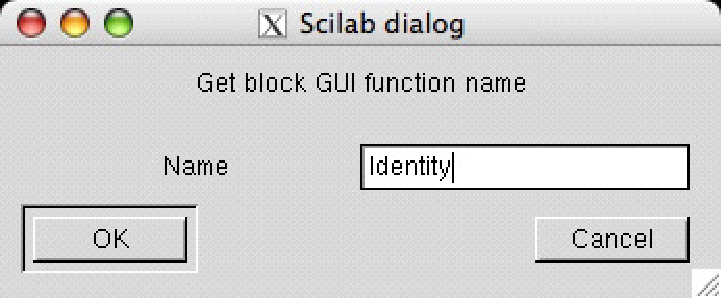
\includegraphics[width=150pt]{../pdf/Scicos-2}
\end{center}
The added block is incorporated in the graphics as in
\begin{center}
    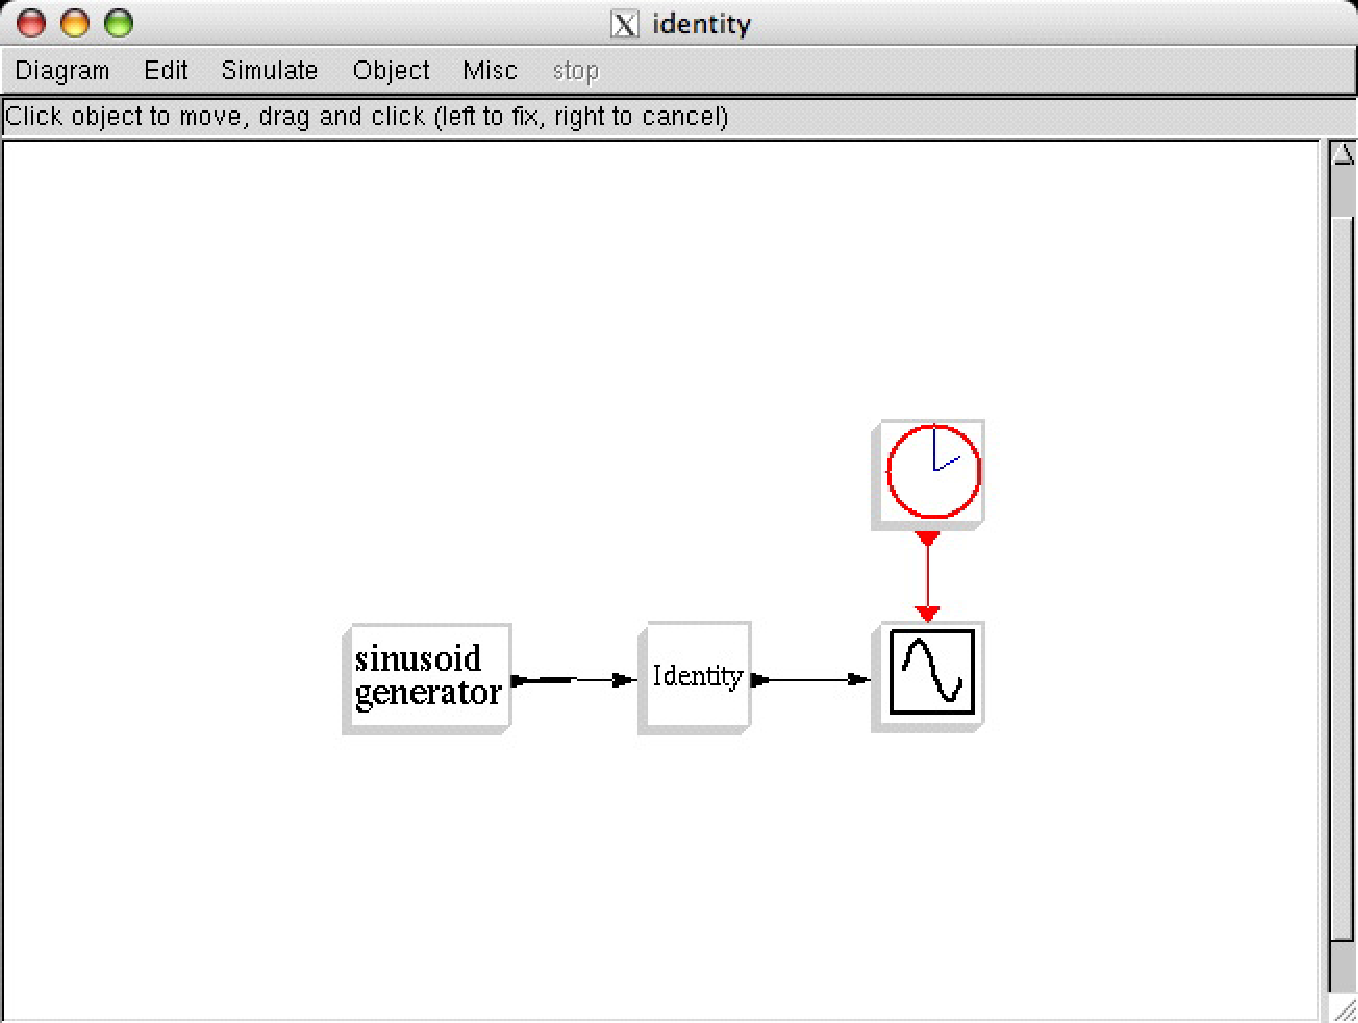
\includegraphics[width=180pt]{../pdf/Scicos-1}
\end{center}
(where the links have been set additionally).

Add the graphics to the the project (using the tab \pp{Scicos models} in
the project panel. Then push the \pp{Run} button. Then Scilab is started
executing a hidden file \pp{.scilab} which loads 
the necessary libraries and the chosen Scicos model automatically.

Note that for development of the synERJY-based block Scicos diagrams should
be saved as text files (using the extension \pp{.cosf}. Then the last version
generated is used for updating the diagram. If the binary version of the
diagram is stored (using the extension \pp{.cos}) the block(s) generated
using \se\  are not updated, but the version of the \se\ block is kept that was
available when the block as been added as a new block. 
This tends to a constant source of confusion when new code has been generated 
by \se\ but no effect can be seen.
 
On Windows, for instance double clicking on one of the Scilab files in the
respective project directory would do the job. Remember that Scicos must be started within the \se\ project directory to load the libraries related to \se.

The support of the \emph{timing} is rather crude in that there are two distinct 
cases only: 
\begin{itemize}
\item either the timing constant is \pp{0sec},
then the sample time of the block will be inherited. 
\item Otherwise one actuator
input is provided. Then according to the paradigms of Scicos the sample
time can be set using a clock source.

\end{itemize}

\emph{Feedtroughs} are detected. However, in contrast to Simulink, the whole
block is flagged to have a feedthrough, which is somewhat more restrictive
than in Simulink, but is a restriction of Scicos.. 

\se\ exception are supported, exception are printed using \pp{sciprint}.
They show in the Scilab window.

Parameters can used. Here the Scicos graphical interface is more convenient 
than the corresponding interface for Sfunctions in that each parameter has a
separate entry.


\paragraph{\textit{\textbf{Warning}}} The method main is ignored when a 
Scicos block is generated. Inspect the method body to check 
whether this may cause problems (often initialisation code can be moved to
the constructor of the configuration class).

\section{The \emph{synERJY} Verification Environment} 

\se\ supports verification, at present on the basis of NuSMV \\
(\pp{http://nusmv.irst.itc.it/}). We use the example \pp{Blink1} (in directory \pp{\$(SE\_HOME/target/examples}) in order to demonstrate the interface. When loaded choose target \pp{Verification}, and the \se-console will change to
\begin{center}
    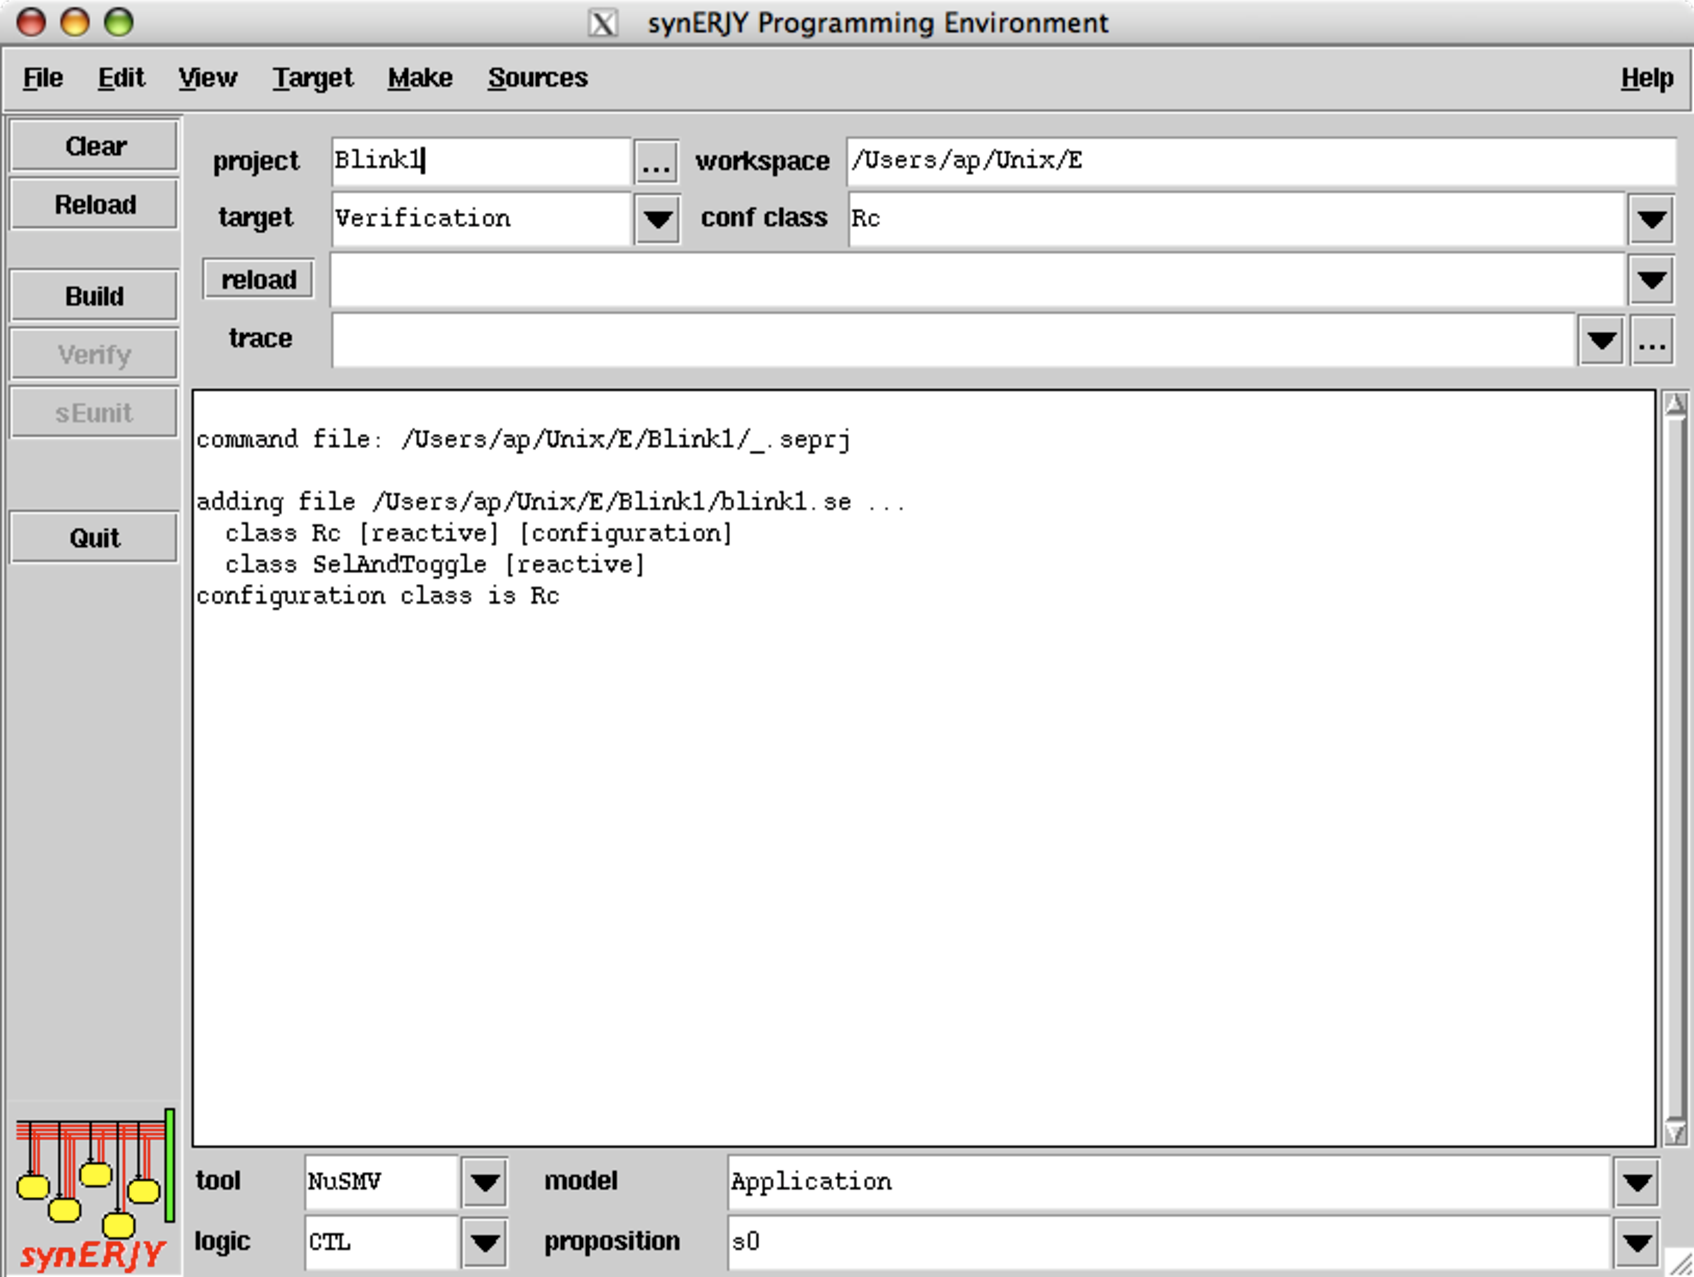
\includegraphics[width=340pt]{../pdf/Verification-console}
\end{center}
At the bottom you see the tool that may be used for verification (at presen t only NuSMV), the logic which may be used to specify the propositions, the scope of the verification (either the full application, or propositions with regard to a specific object), and one may choose the proposition to prove using labels. Pressing the \pp{Build} button generates the model, and then pressing the \pp{Verification} button starts the verification. Prerequisite is that the path to NuSMV has been defined as environment variable.

\paragraph{Warning:} This has only been tested for a view examples on Unix systems (actually for OS X). This binding is of alpha Status.

\section{How to Make \emph{synERJY} Available for a New Micro-controller}

This description shows the steps of building the runtime environment for a new micro-controller.

\begin{itemize}
\item \textit{\textbf{Choose a name for the new type of micro controller}}.
      In this description we refer to this name by
        \texttt{mcuname}.
        
\item  \textit{\textbf{Describe how to install the tools necessary to 
       build applications}}.\\
       Typically these tools are:
        \begin{itemize}
            \item a C-compiler and its development environment,
            \item an upload tool, to install software into a target system.
        \end{itemize}
        
\item \textbf{\textit{Create a a subdirectory-tree to} \texttt{\$SE\_HOME/target}}.
      \begin{verbatim}
       cd $SE_HOME/target
       mkdir mcuname
       cd mcuname
       mkdir src
       mkdir include
       mkdir lib
       mkdir lib/src
       mkdir examples
    \end{verbatim}
The directories in \texttt{\$SE\_HOME/target/mcuname/} should hold the following files (compare, e.g.,  \texttt{\$SE\_HOME/target/AT90s8515/}):
\BEP
src/                     \texttt{*.se} \textit{files to utilise the installation
                         Typically the directory holds these
                         files with basic target classes.}
                       
   Mcu.se                \textit{\se-classes that provide access 
                         kernel of the micro controller unit.
                         These classes may
                           - define constants
                          - basic facilities like interrupt
                            enable/disable
                          - storage access
                          - addresses of registers, 
                            peripheral units}
                        
   StdReader.se          \textit{serial input of a character stream}
   StdBufferdReader.se   \textit{line buffered serial input}
   StdWriter.se          \textit{serial output of a character stream}
   StdBufferdWriter.se   \textit{line buffered serial output}                        
   Realtime.se           \textit{access of the basic realtime clock}

include/                 \textit{target specific C-header files,
                            makefile-include-files ...}

lib/libsert.a            \textit{the target specific runtime library}

lib/src/                 \textit{sources to build the runtime library}

examples/                \textit{\se\ classes as examples,
                            for instance to show
                            the facilities of the classes in }
                            src/*.se
\EEP
                    
\item \textbf{\textit{Provide Basic functions and C-macros for the runtime environment
}}

    \begin{enumerate}
        \item[a)] \textit{Functions for the Timing of the Synchronous Engine.}
        
        Prototypes of these functions are defined in
        \begin{quote}
           \texttt{\$SE\_HOME/include/se\_realtm.h}.
        \end{quote}
         They  should be implemented as a single C-module in the file
        \begin{quote}
           \texttt{\$SE\_HOME/target/lib/src/se\_realtm.c}.
        \end{quote}
        
       \item[b)] \textit{Functions and Macros for Using IOstreams for 
            Input and Output.}
            
       Typically these are facilities implemented by
          \begin{itemize}
              \item \texttt{<stdio.h>} on operating systems, or
              \item using asynchronous serial units (e.g. UART) 
                of micro-controllers
           \end{itemize}
        Use

          \begin{quote}
            \texttt{\$SE\_HOME/target/mcuname/include/target.h}
          \end{quote}

        to define C-function-prototypes and -macros, that are to be included
        in order to access the implementation of the basic target classes.
        Since the interfaces are defined by \se\-types, the file target.h
        must \#include <se\_types.h>


      \item[c)] \textit{Provide the Implementation for Each Function as 
            Declared in} \texttt{target.h}
            
             in a individual C-file of the directory
          \begin{quote}
             \$SE\_HOME/target/mcuname/lib/src/
          \end{quote}

            Thus function is compiled into an individual C-module.
            Linkage will only insert function implementations into the
            target binary, which are actually used in the application.
  \end{enumerate}

\item \textit{\textbf{Provide a}} \texttt{Makefile} \textit{\textbf{to Build 
      the Runtime Library}}
      
      The makefile is
      \begin{quote}
          \texttt{\$SE\_HOME/target/mcuname/lib/Makefile}
      \end{quote}
      The first rule of this makefile must produce the runtime library
      The makefile is
      \begin{quote}
          \texttt{\$SE\_HOME/target/mcuname/lib/libse.rt.a}
      \end{quote}
        
\item \textit{\textbf{Provide a}} \texttt{Makefile} \textit{\textbf{for
      Writing Makefiles for Applications}}
      
      The makefile is
      \begin{quote}
          \texttt{\$SE\_HOME/target/include/Makefile.inc}
      \end{quote}
      This makefile should provide definitions to access
      \begin{itemize}
         \item the C-compiler, linker, and other tools,
         \item  the runtime libraries of the C-development environment,
         \item  other tools like the upload program, and
         \item  the specific \se\-runtime library
     \end{itemize}
   Typically default rules for compilation, linking and uploading
    are defined. These definitions should support writing of application
    specific makefiles.


\item \textbf{\textit{Give application examples, that also test the proper installation
}}

    There are two example applications in 
      \begin{quote}
          \$SE\_HOME/target/mcuname/examples/
      \end{quote}
        

            McuTiming.se

    Adapt these examples to the micro-controller and its environment.
    Compile and run them to check the proper installation.

\end{itemize}


\begin{thebibliography}{9}

\bibitem{esterel} G.~Berry and G.~Gonthier.  The \textsc{Esterel}
synchronous programming language: design, semantics, implementation.
{\em Science of Computer Programming}, 19(2):87--152, 1992.

\bibitem{halbwachs} N.~Halbwachs.  {\em Synchronous Programming of
Reactive Systems}, Kluwer Academic Publishers, Dordrecht, 1993.

\bibitem{statecharts} D.~Harel. Statecharts: A visual approach to
complex systems, \emph{Science of Computer Programming}, 8:231--274, 1987.

\bibitem{lustre} N.~Halbwachs, P.~Caspi, P.~Raymond, and D.~Pilaud.
The synchronous dataflow programming language Lustre.
{\em Proceedings of the IEEE}, 79(9):1305--1320, 1991.

\bibitem{Matlab}  \texttt{www.mathworks.com}

\bibitem{Scilab} \texttt{www.scilab.org}

\end{thebibliography}


\end{document}

